\subsection{安装 Ubuntu 操作系统}

如果你只需要处理一般的事务,打游戏,那么你不需要了解下面这些了。
但是其实世界上的大多数科学家和工程师几乎用的都是 Linux 系统作为他们的电脑工具。
就因为它简单,可靠,稳定,强大,有趣。
甚至很多时候 Linux 就是唯一的选择。
Ubuntu 作为当下非常流行的 Linux 发行版,
在桌面办公、服务器方面都有着不俗的表现。
在接触一个新的系统之前,学会安装是深入了解它的前提。

使用一个 Linux 操作系统的方式有很多,常见的有虚拟机和双系统两种方式。
这里我们主要介绍一下双系统 (Win10 + Ubuntu) 的安装。

\begin{itemize}
	\item [I.] 准备工作
		\begin{itemize}
			\item [I-a.] 磁盘分区:
			    首先查看本机的磁盘情况(win+x $\to$ Disk Management)。
				在足够大的硬盘上选择合适的大小进行压缩(右键$\to$Shink Volume),
				压缩卷的大小即为即将安装的Ubuntu系统的大小,推荐为60GB以上(建议120GB)。
				压缩后磁盘出现空白卷,如图 (\ref{fig:shrinkVol})
				\begin{figure}[htbp]
					\centering
					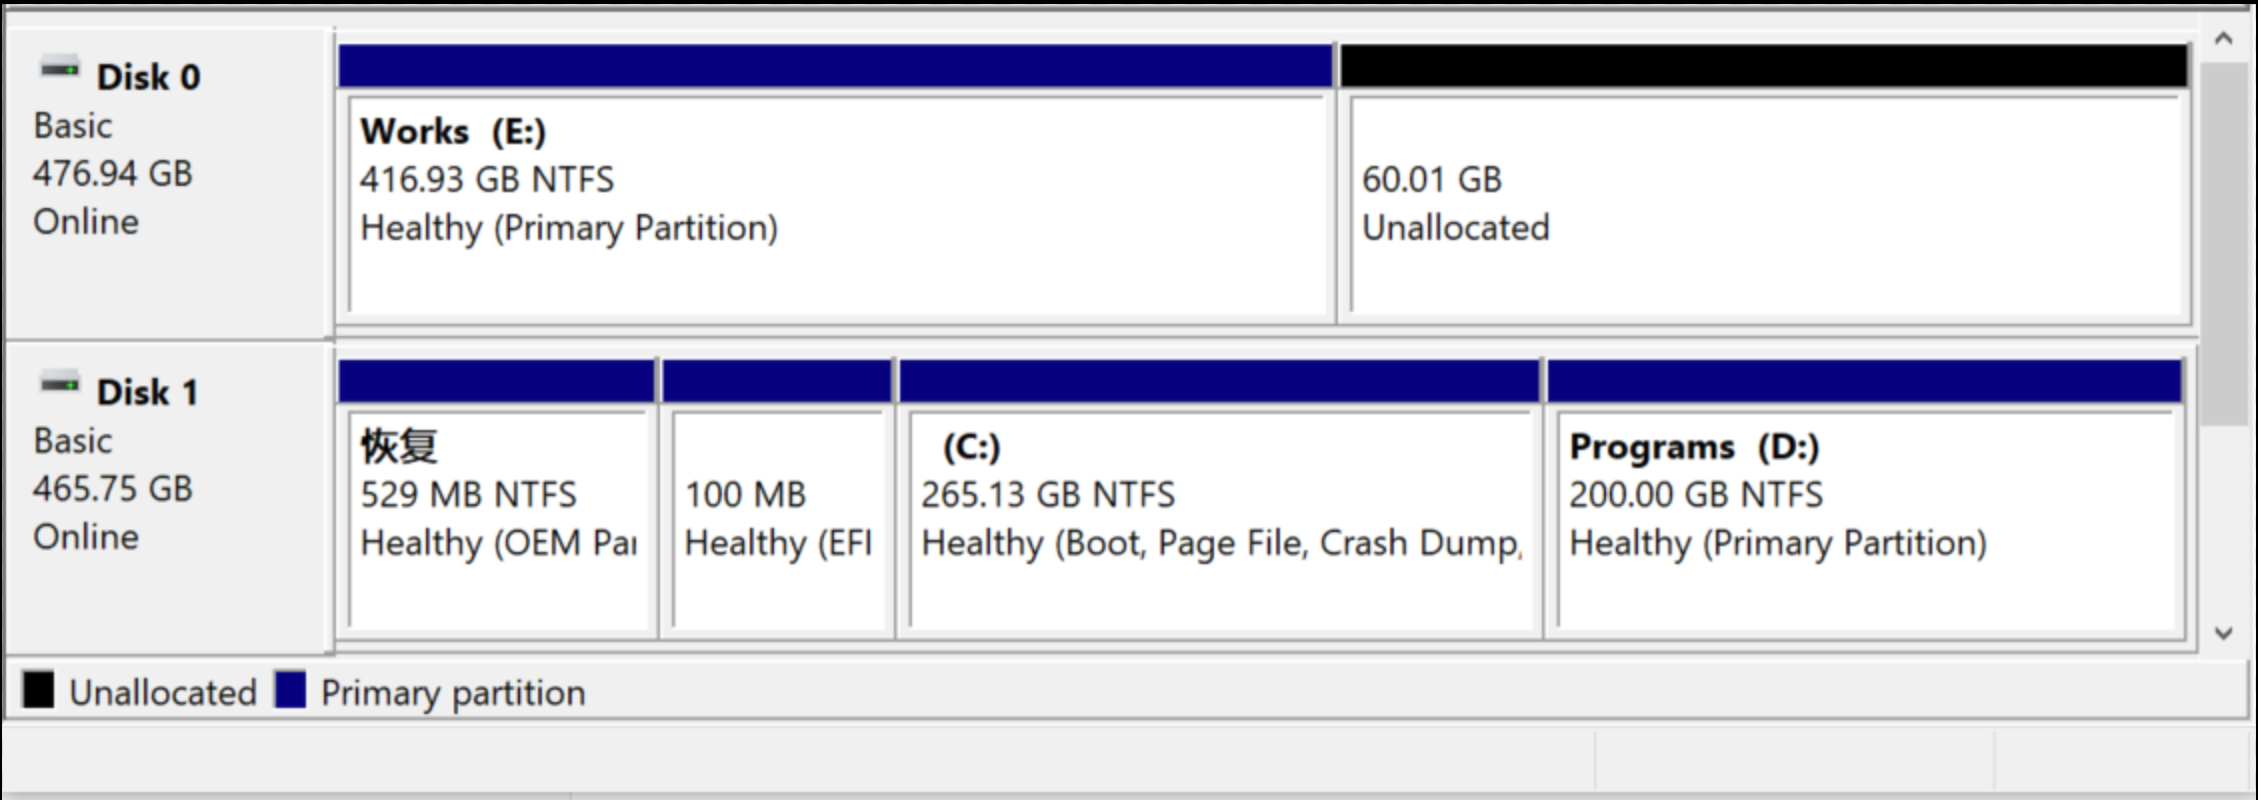
\includegraphics[width=0.7\textwidth]{png/shrinkVol}
					\caption{压缩后的磁盘出现空白卷(Unallocated)。}
					\label{fig:shrinkVol}
				\end{figure}
			\item [I-b.] 下载系统镜像:从 Ubuntu 官网下载最新安装镜像,
				下载地址为
				\begin{verbatim}
				https://ubuntu.com/download/desktop.
				\end{verbatim}
				\begin{figure}[htbp]
					\centering
					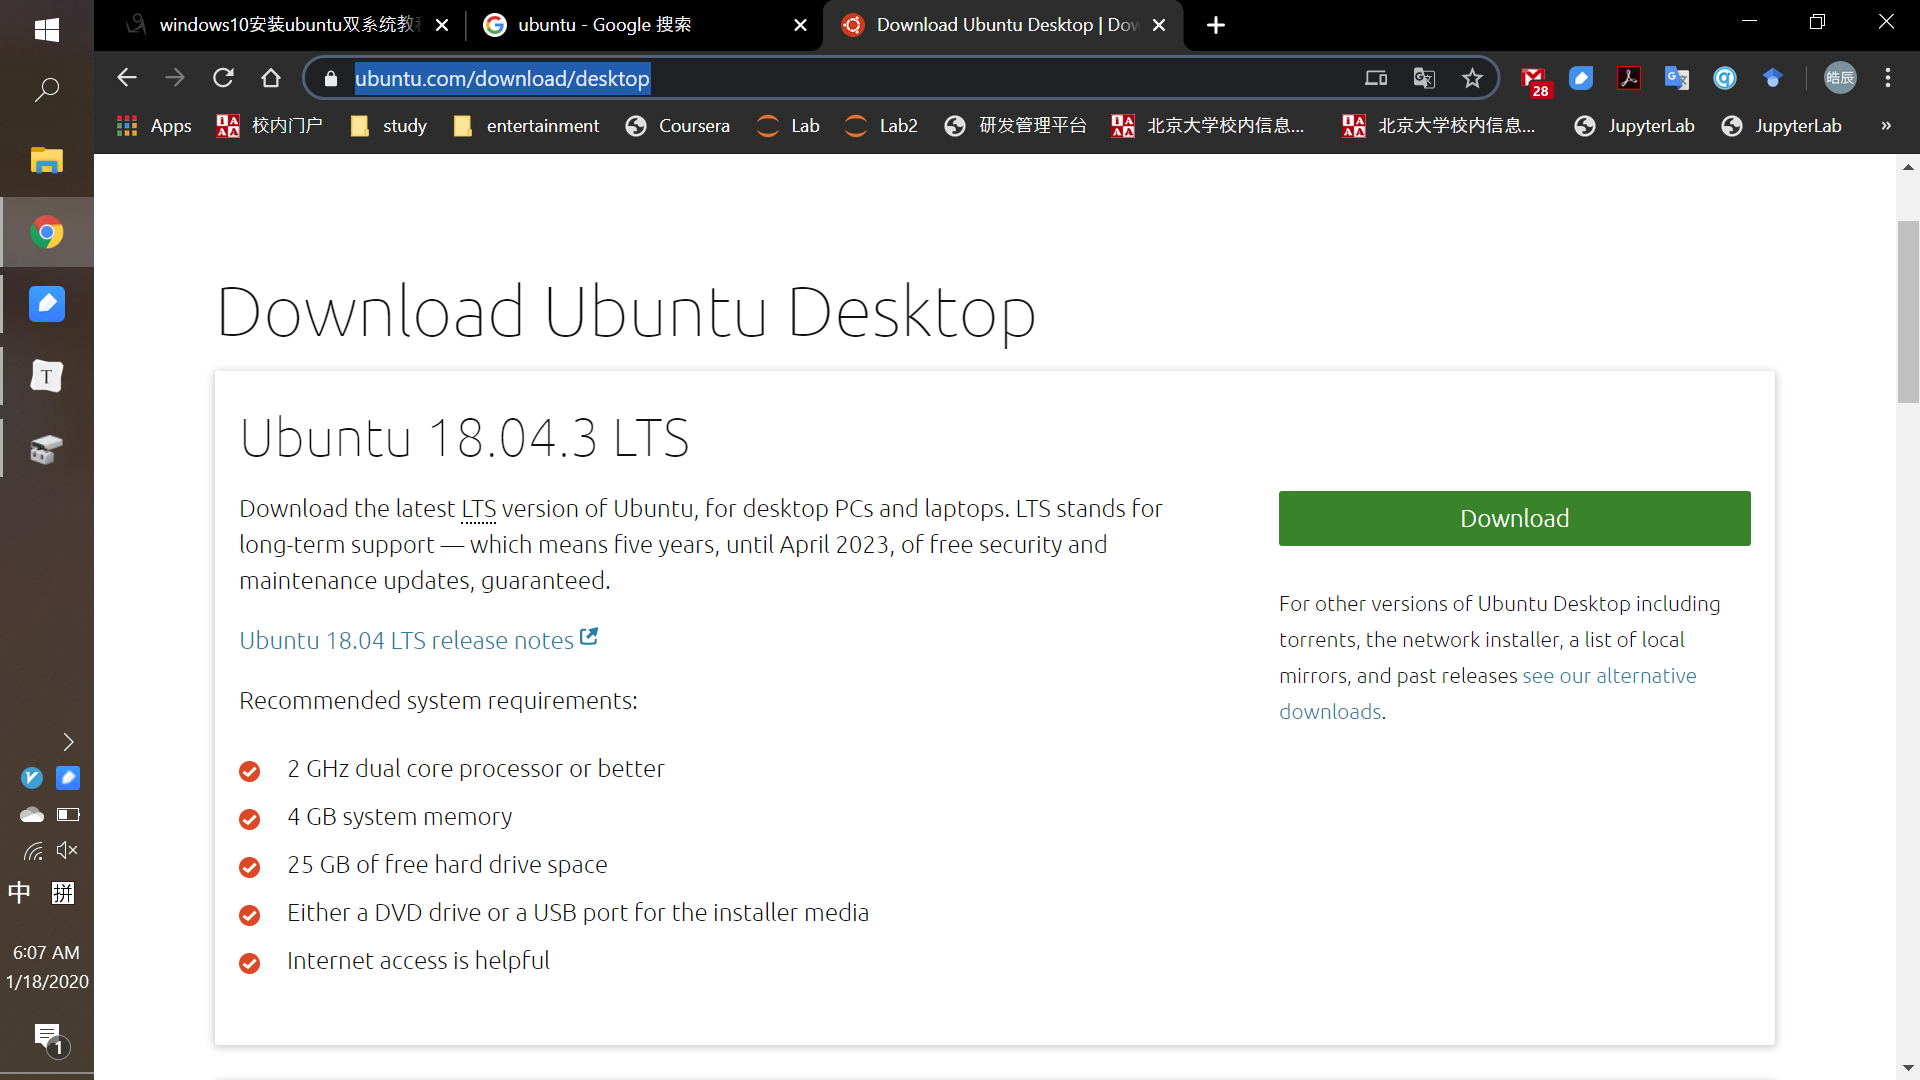
\includegraphics[width=0.7\textwidth]{png/ubuntuDown}
					\caption{Ubuntu 操作系统下载网址。}
					\label{fig:ubuntuDown}
				\end{figure}
			\item [I-c.] 制作启动盘:当系统镜像下载好之后,需要一个新的4G以上的u盘。
				接着下载启动盘制作工具 UltraISO ( \url{https://cn.ultraiso.net/xiazai.html})。
				该软件为免费试用版,下载好之后安装即可(最后一步点击继续试用)。
				接着在 UltraISO 中制作启动盘:
				\begin{itemize}
					\item 打开之前下载的 Ubuntu 镜像文件(文件$\to$打开);
					\item 选择写入硬盘镜像(启动$\to$写入硬盘镜像)。
				\end{itemize}
				注意写入过程中会格式化u盘。
			 	\begin{figure}[htbp]
			 		\centering
			 		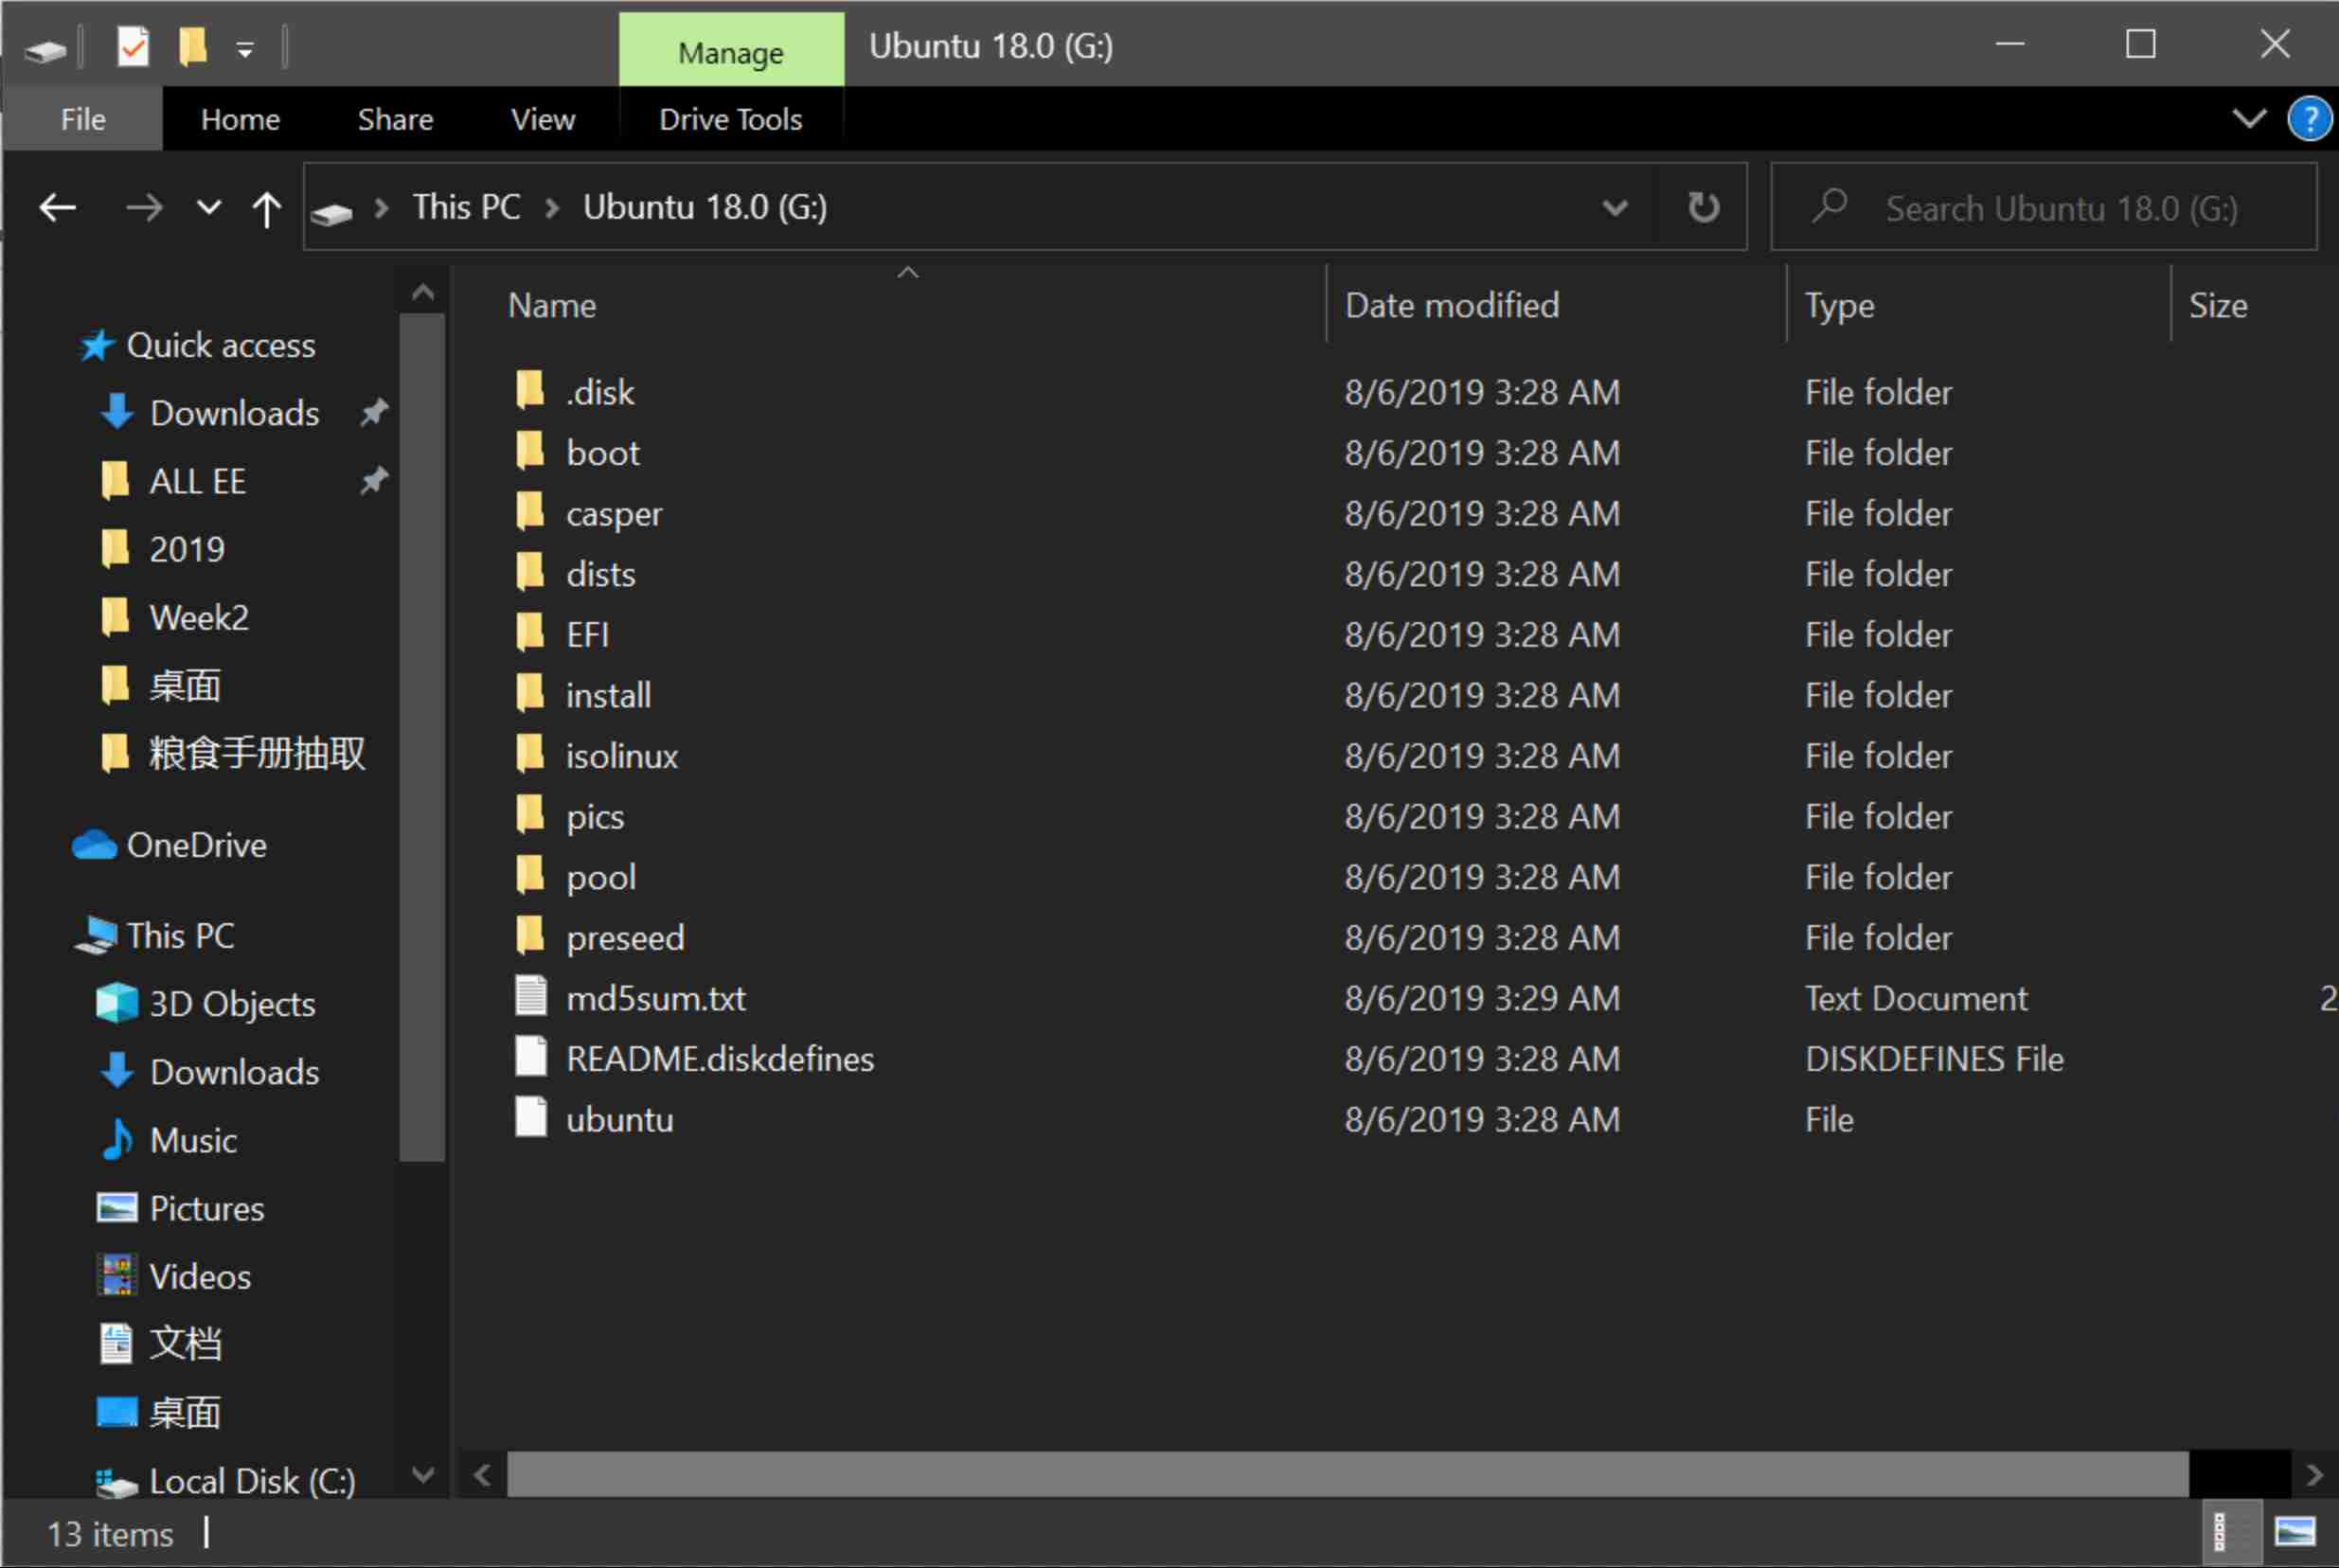
\includegraphics[width=0.75\textwidth]{png/UltraISO}
			 		\caption{制作完成后的启动盘。}
			 		\label{fig:UltraISO}
			 	\end{figure}
		\end{itemize}

	\item [II.] 安装工作
		\begin{itemize}
			\item [II-a.] 关闭所有程序后,插入制作好的启动盘,重新启动电脑,
				并且在启动出现提示时按 F12(不同电脑不同)键进入 boot 选项,
				选择对应的启动盘作为启动介质(将 USB 移动到最上面),
				然后按 F10 保存并退出,接着选择安装 Ubuntu。
				\begin{figure}[htbp]
					\centering
					\subfigure[将启动盘作为首选启动项]{
						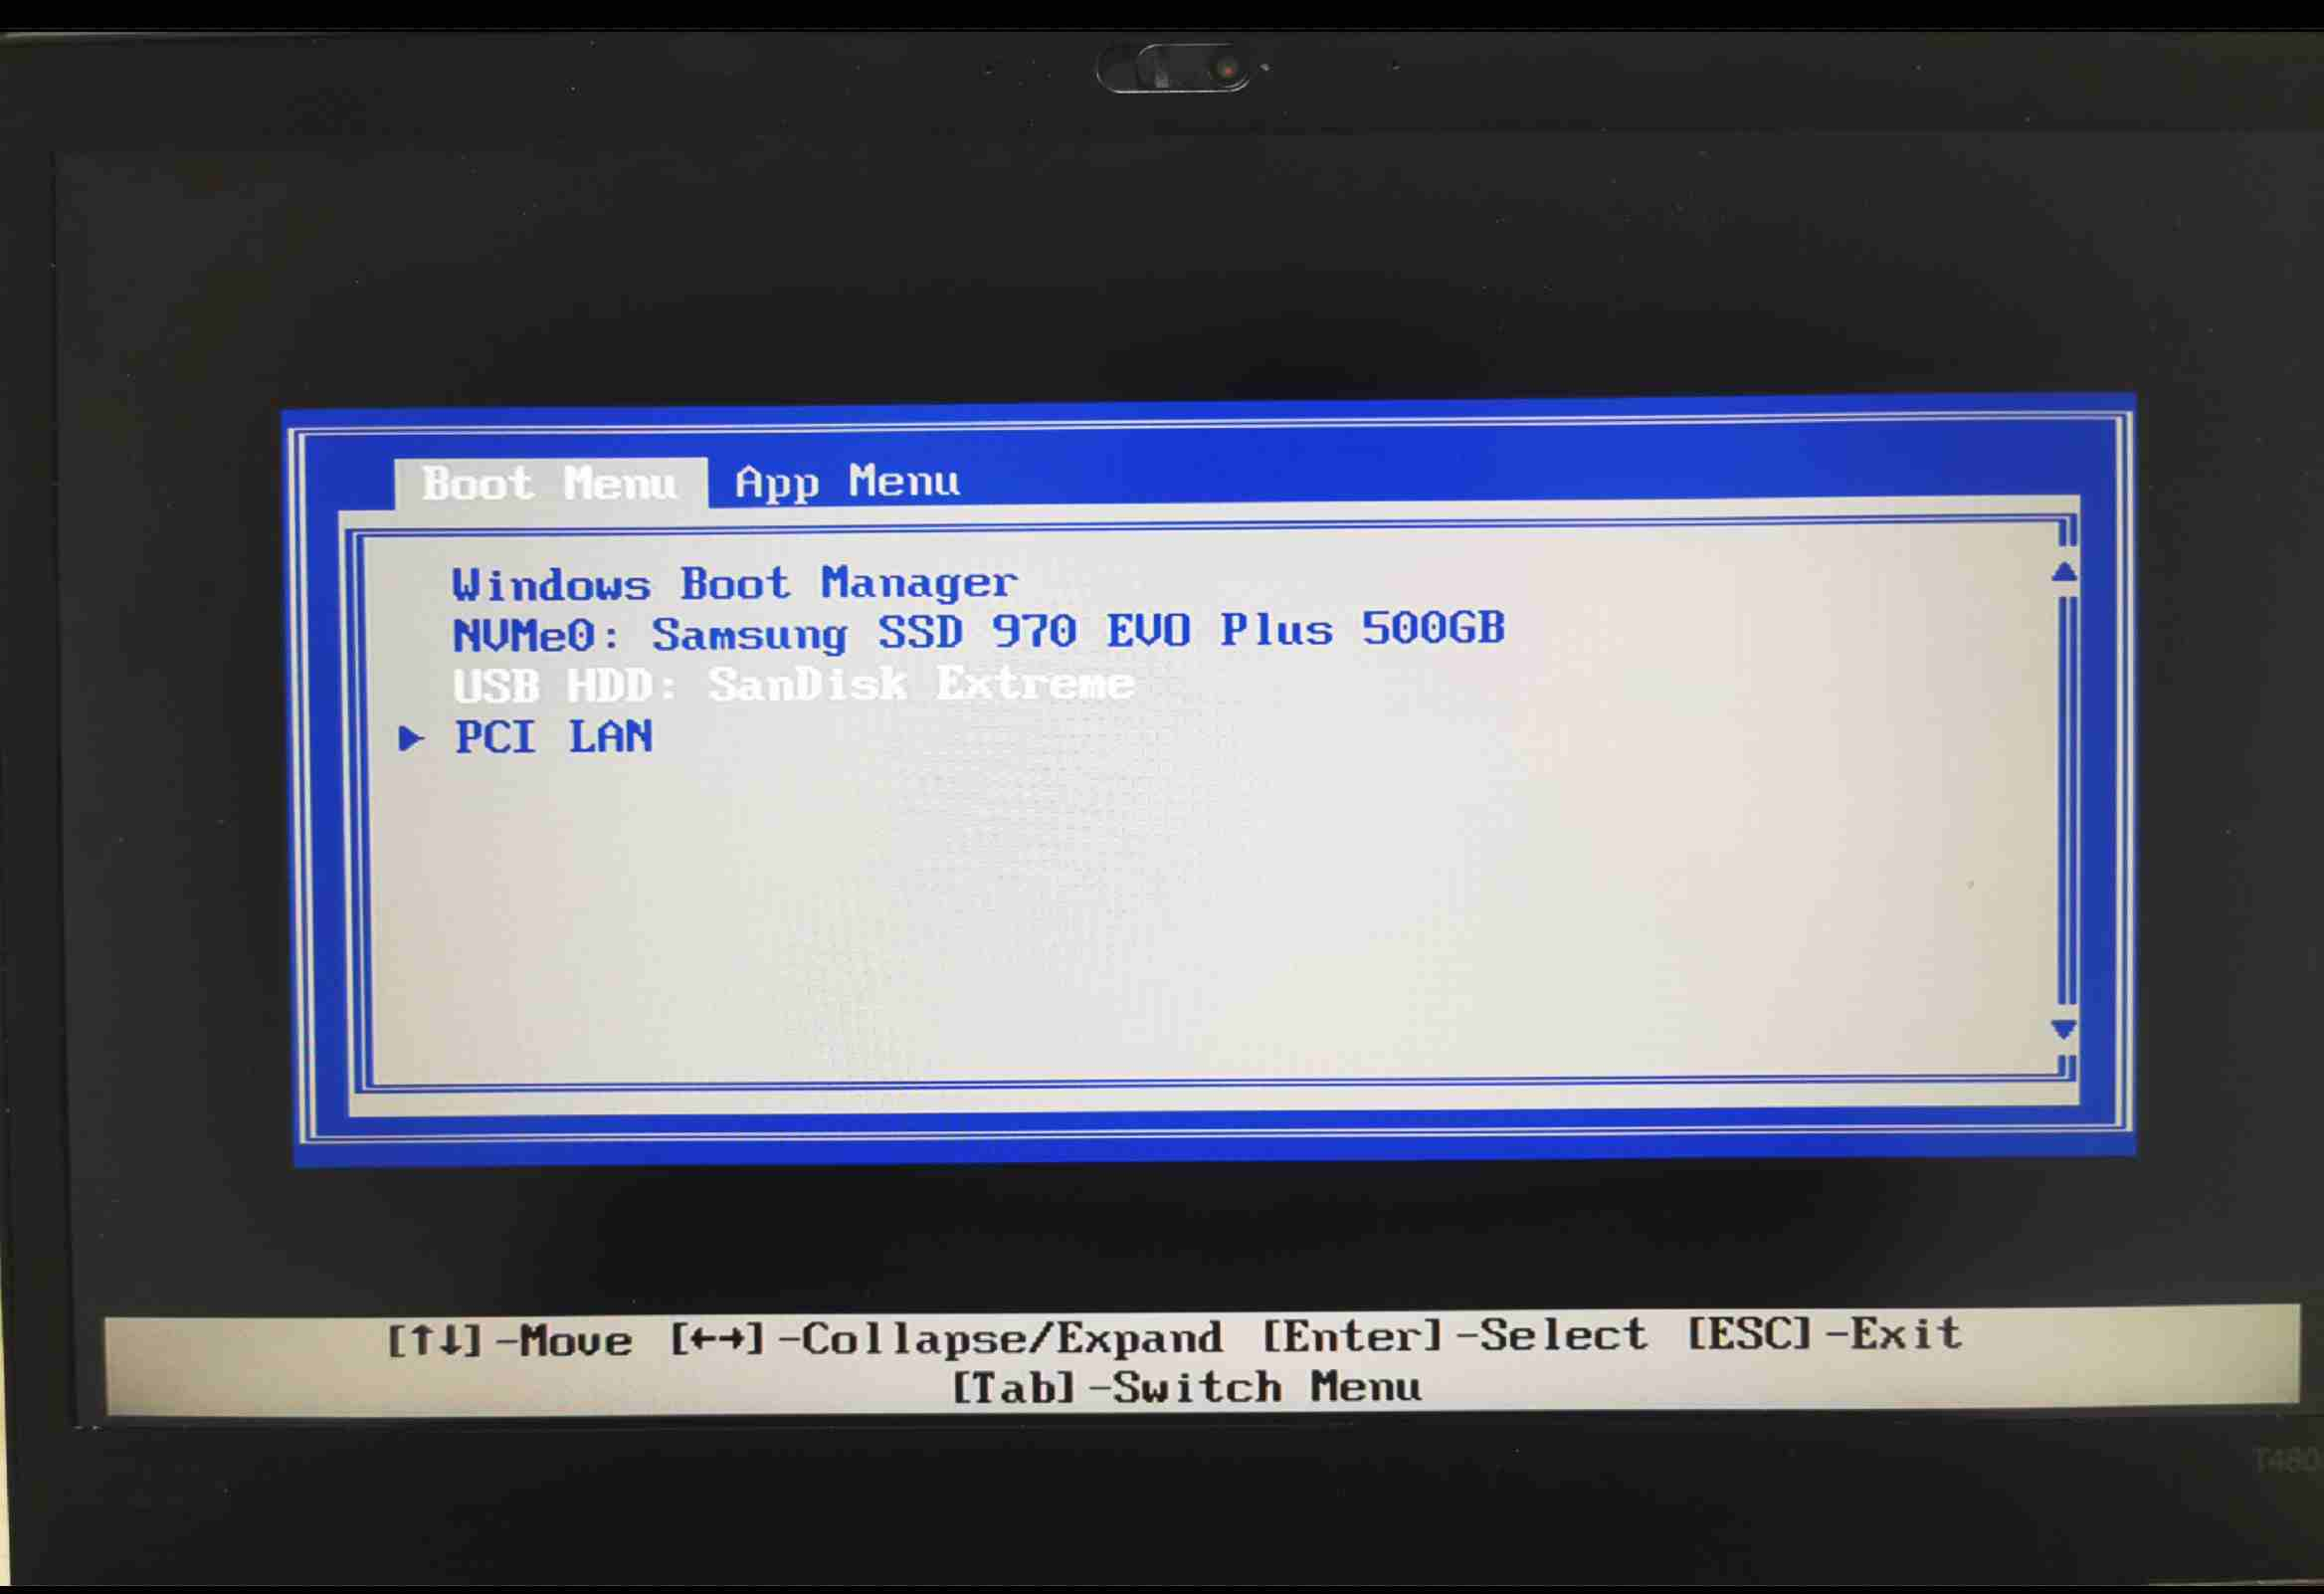
\includegraphics[width=0.42\linewidth]{png/bootMenu}
					}
					\hfill
					\subfigure[选择安装Ubuntu]{
						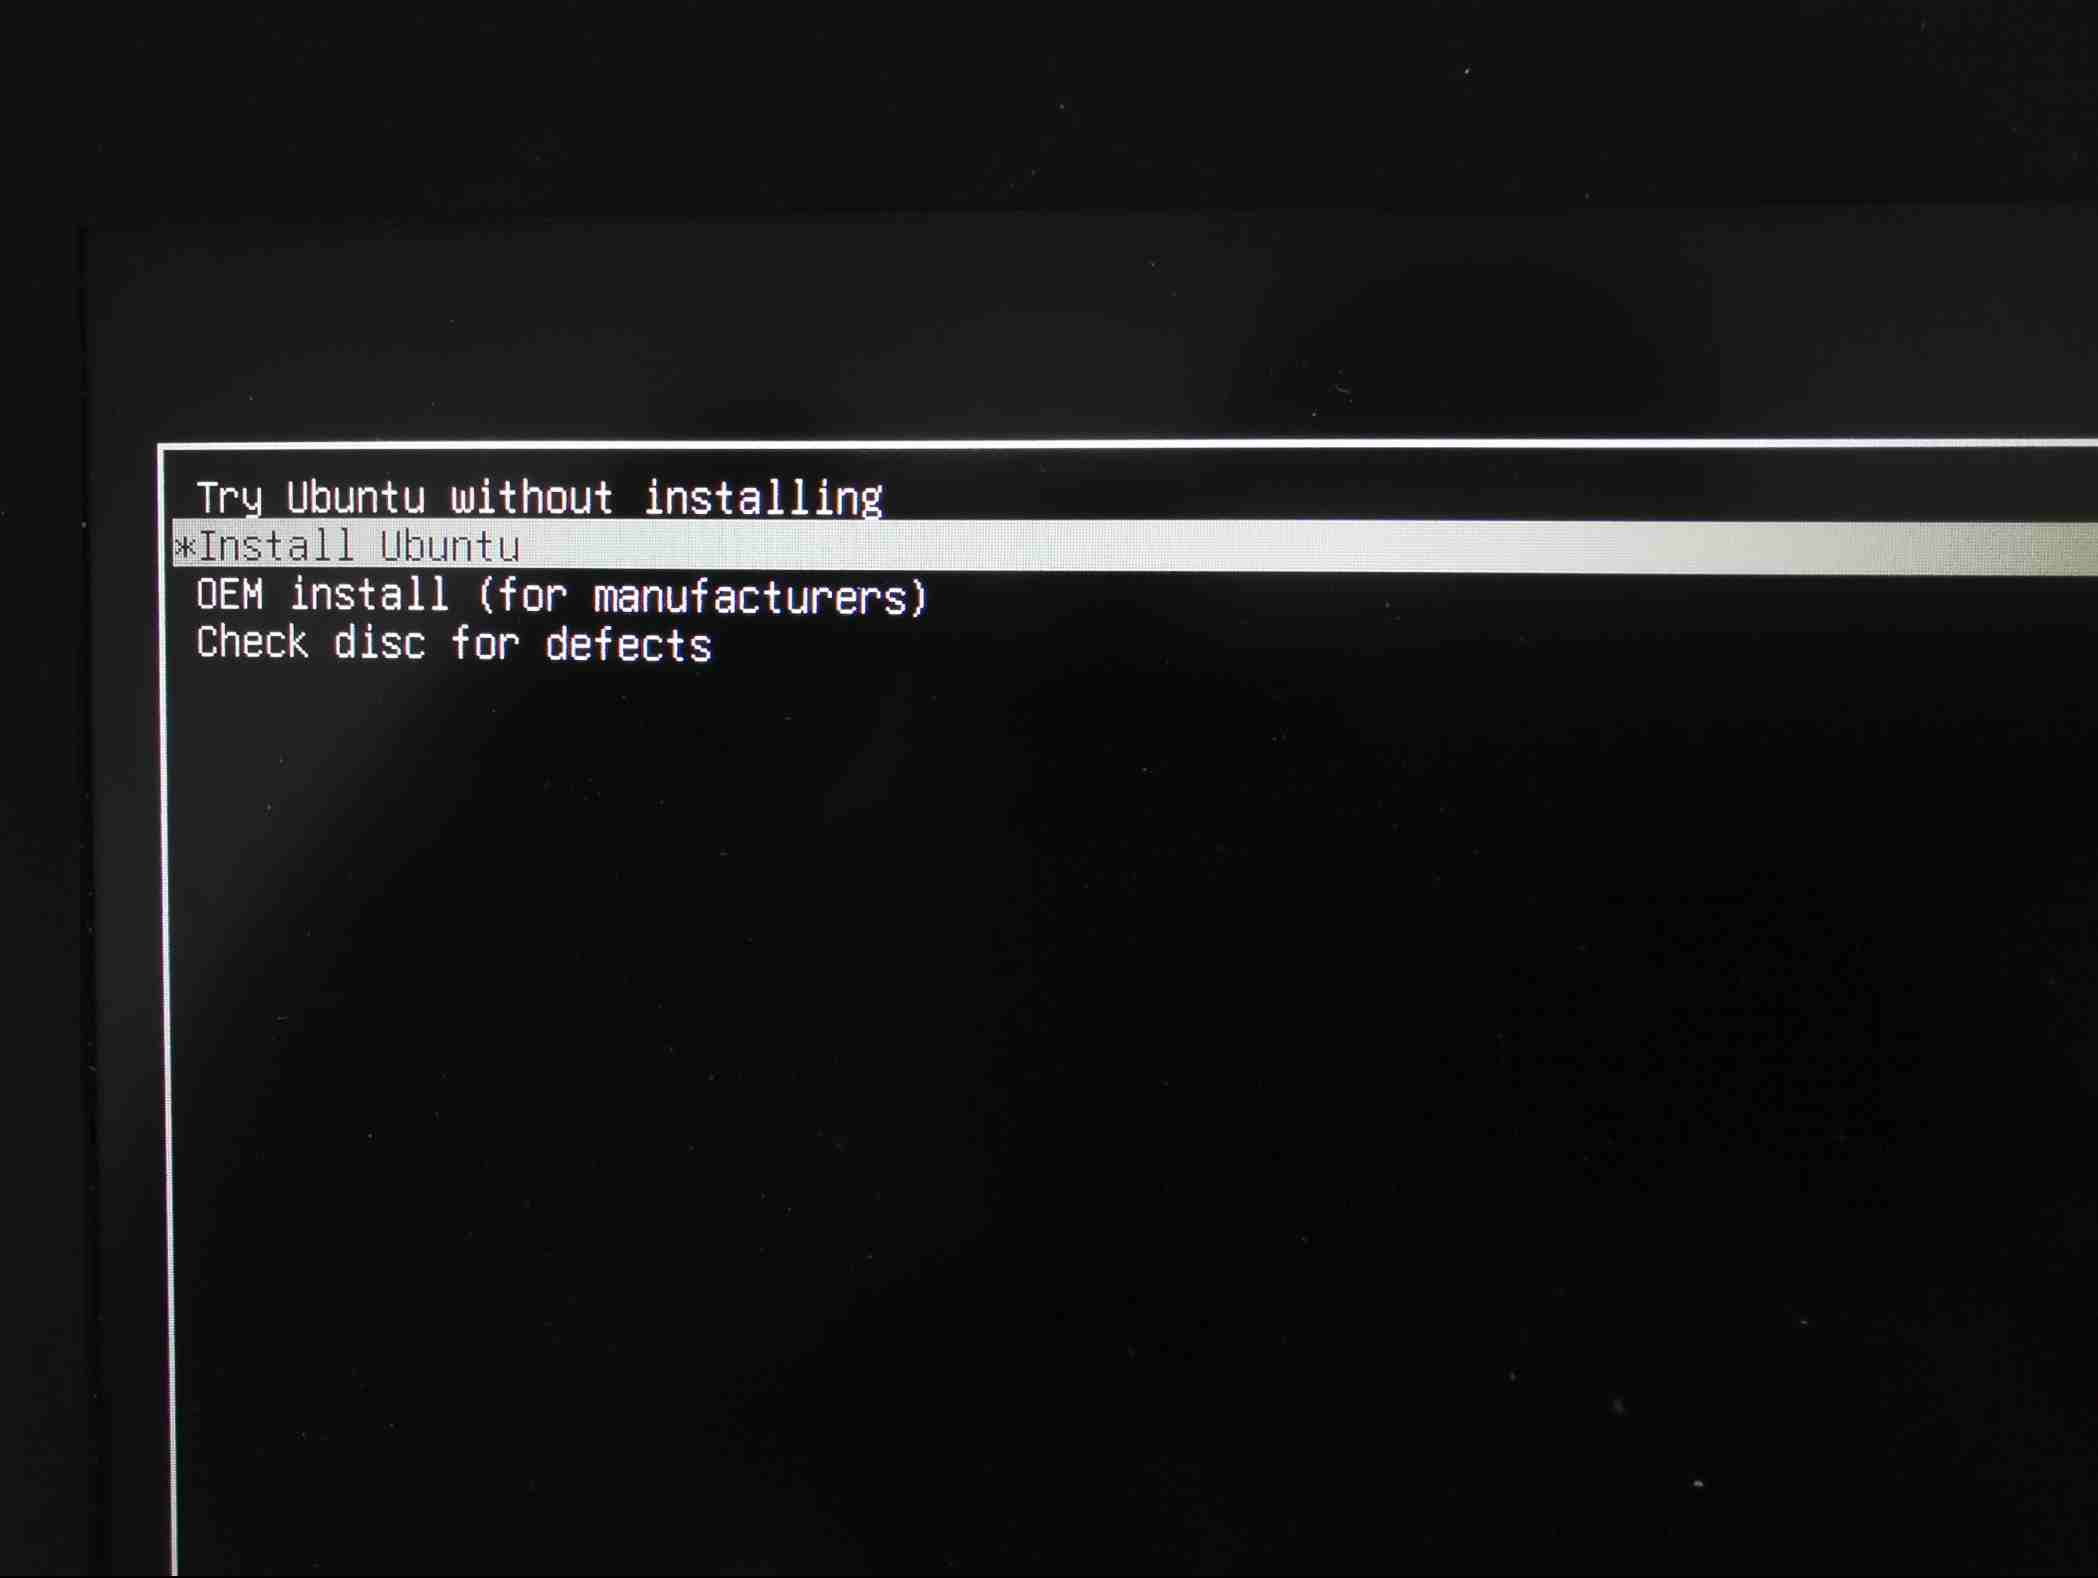
\includegraphics[width=0.42\linewidth]{png/InstallUbuntu}
					}
					\label{fig:UbuntuInstall}
				\end{figure}
			
				如果没有直接进入到 boot 选项的快捷键,可先进入 bios 界面,
				然后切换到 boot 选项进行设置,
				不同型号不同品牌的电脑可能会稍有差异。
			\item [II-b.] 接着选择合适的语言和键盘布局,正常安装、一路下一步后直到安装类型界面,
				此时选择其他选项进入系统分区,选中之前压缩磁盘得到的空闲硬盘空间,
				选择左下角的 + 号依次添加四个分区:
				\begin{itemize}
					\item 系统分区,即存放Ubuntu系统的分区
					(大小20GB,主分区,空间起始位置,Ext4文件系统,挂载点/);
					\item 交换分区,即内存交换空间,一般和本机内存大小相同
					(大小16GB,逻辑分区,空间起始位置,交换空间);
					\item boot分区,即启动文件分区
					(大小200M/400M,逻辑分区,空间起始位置,Ext4文件系统,挂载点/boot);
					\item 用户分区,即真正使用的剩余空间,将空余的硬盘全部分配
					(大小为剩下全部,逻辑分区,空间起始位置,Ext4文件系统,挂载点/home)。
				\end{itemize}
				\begin{figure}[htbp]
					\centering
					\subfigure[语言键盘设置]{
						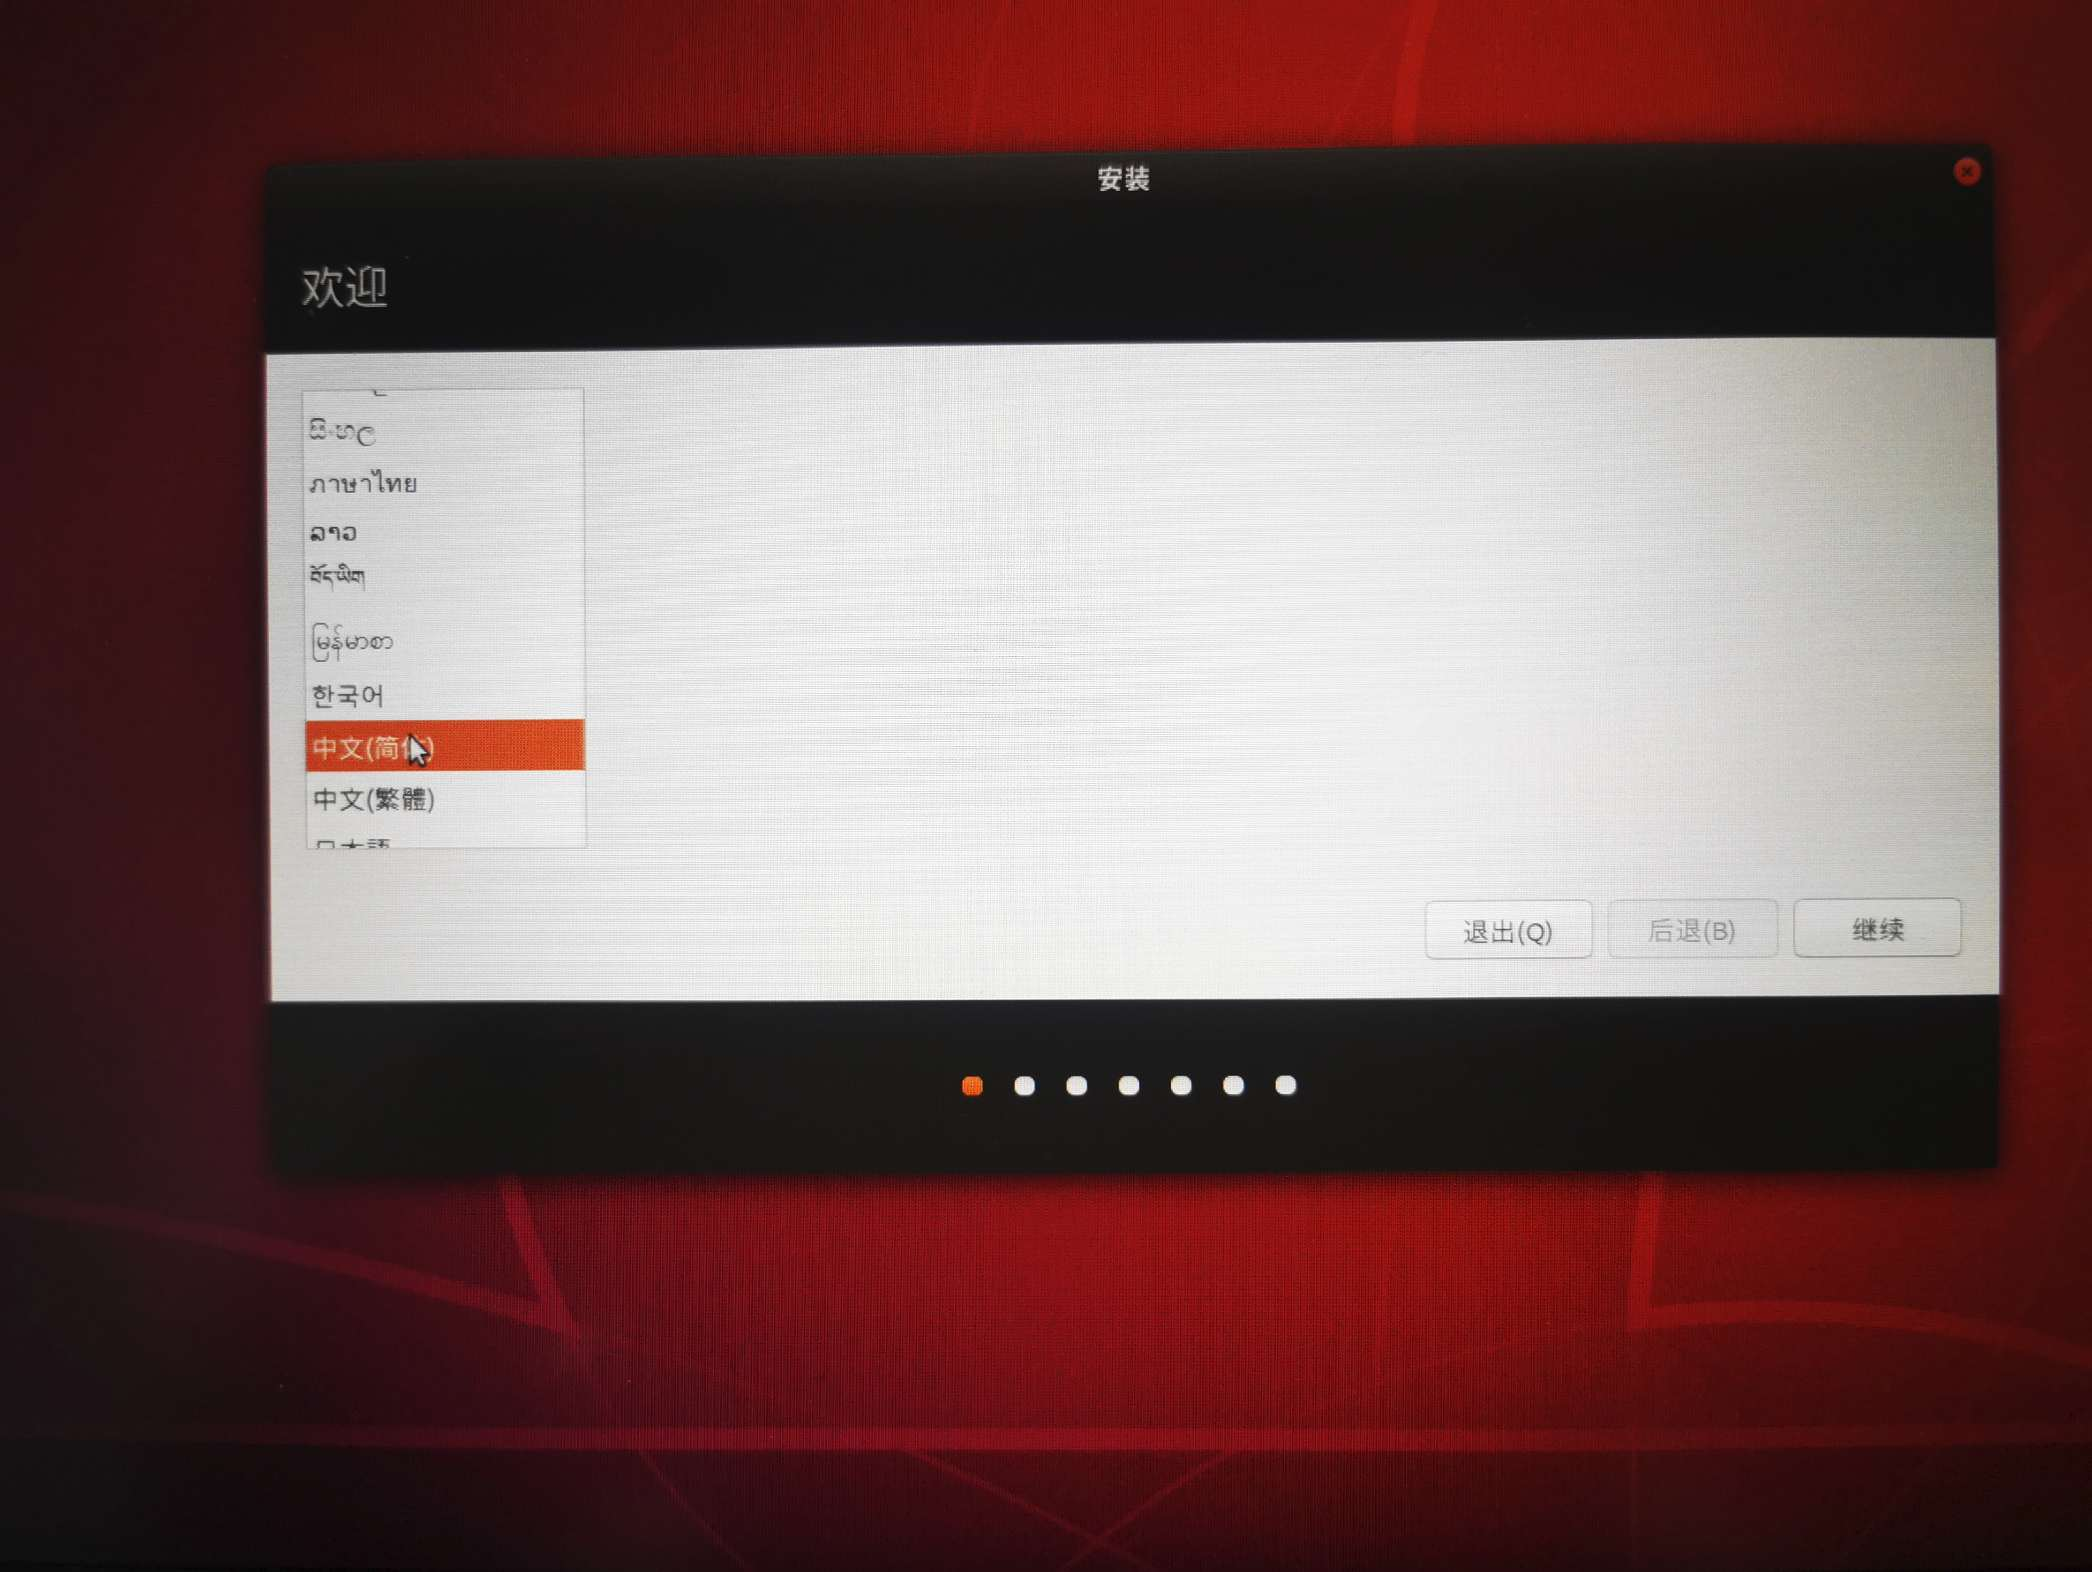
\includegraphics[width=0.42\linewidth]{png/language}
					}
					\hfill
					\subfigure[安装类型]{
						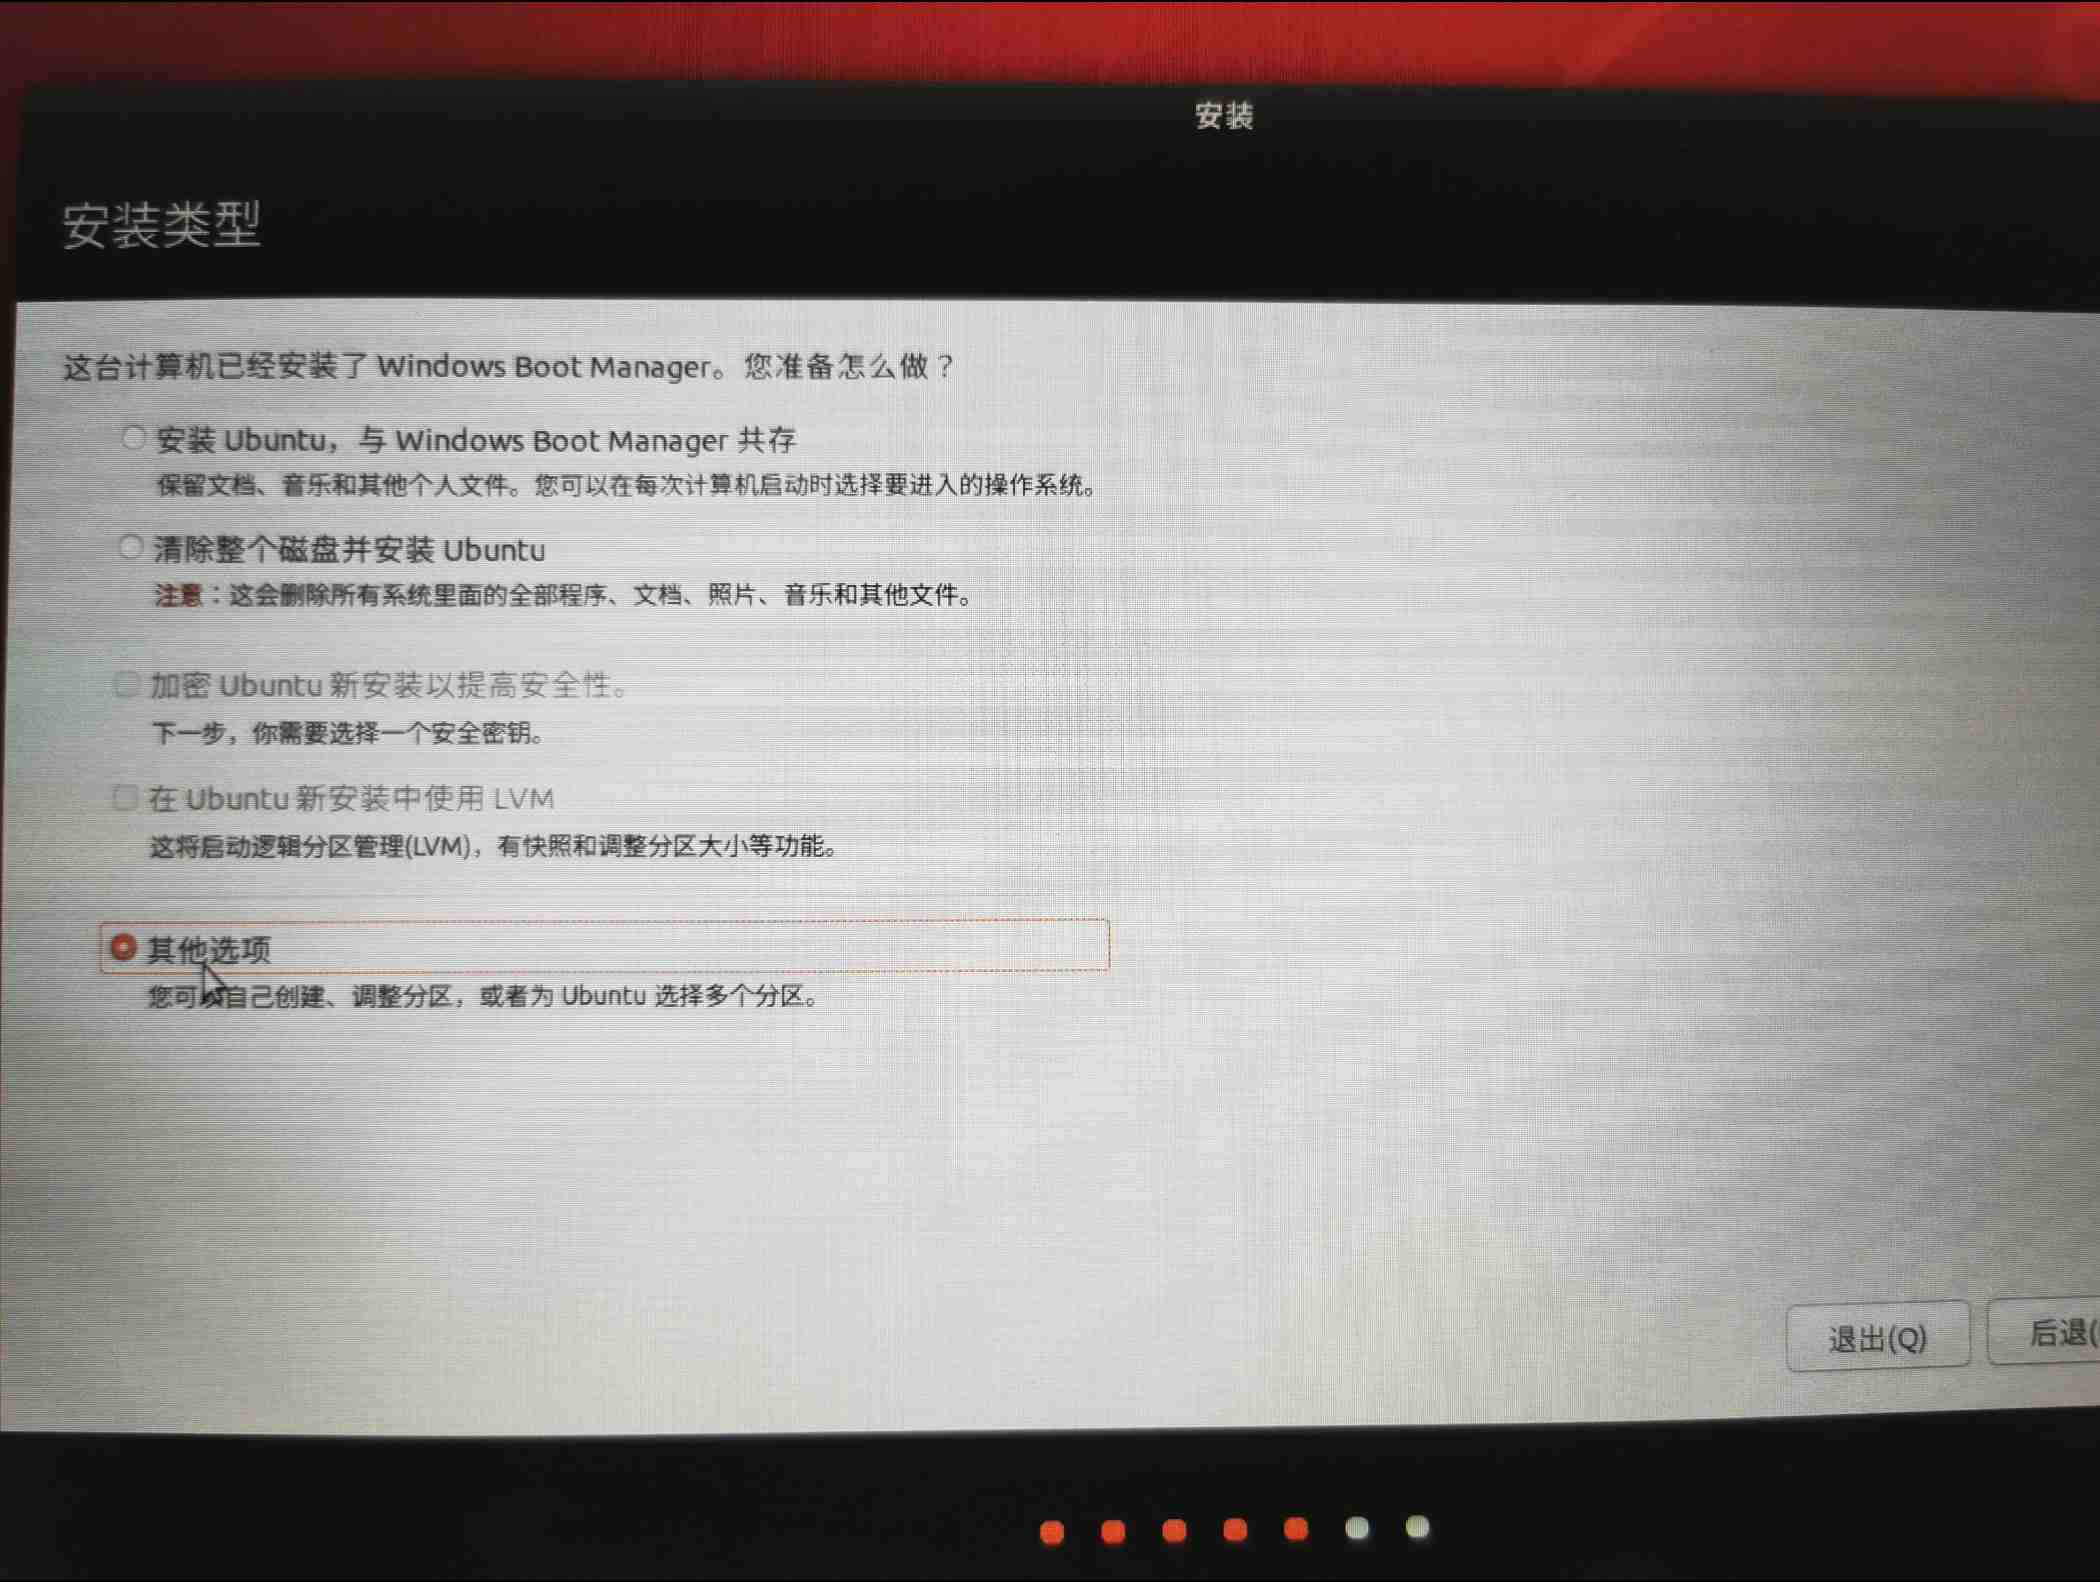
\includegraphics[width=0.42\linewidth]{png/InstallType}
					}
					\label{fig:installType}
  				\end{figure}
				\begin{figure}[htbp]
					\centering
					\subfigure[系统分区设置]{
						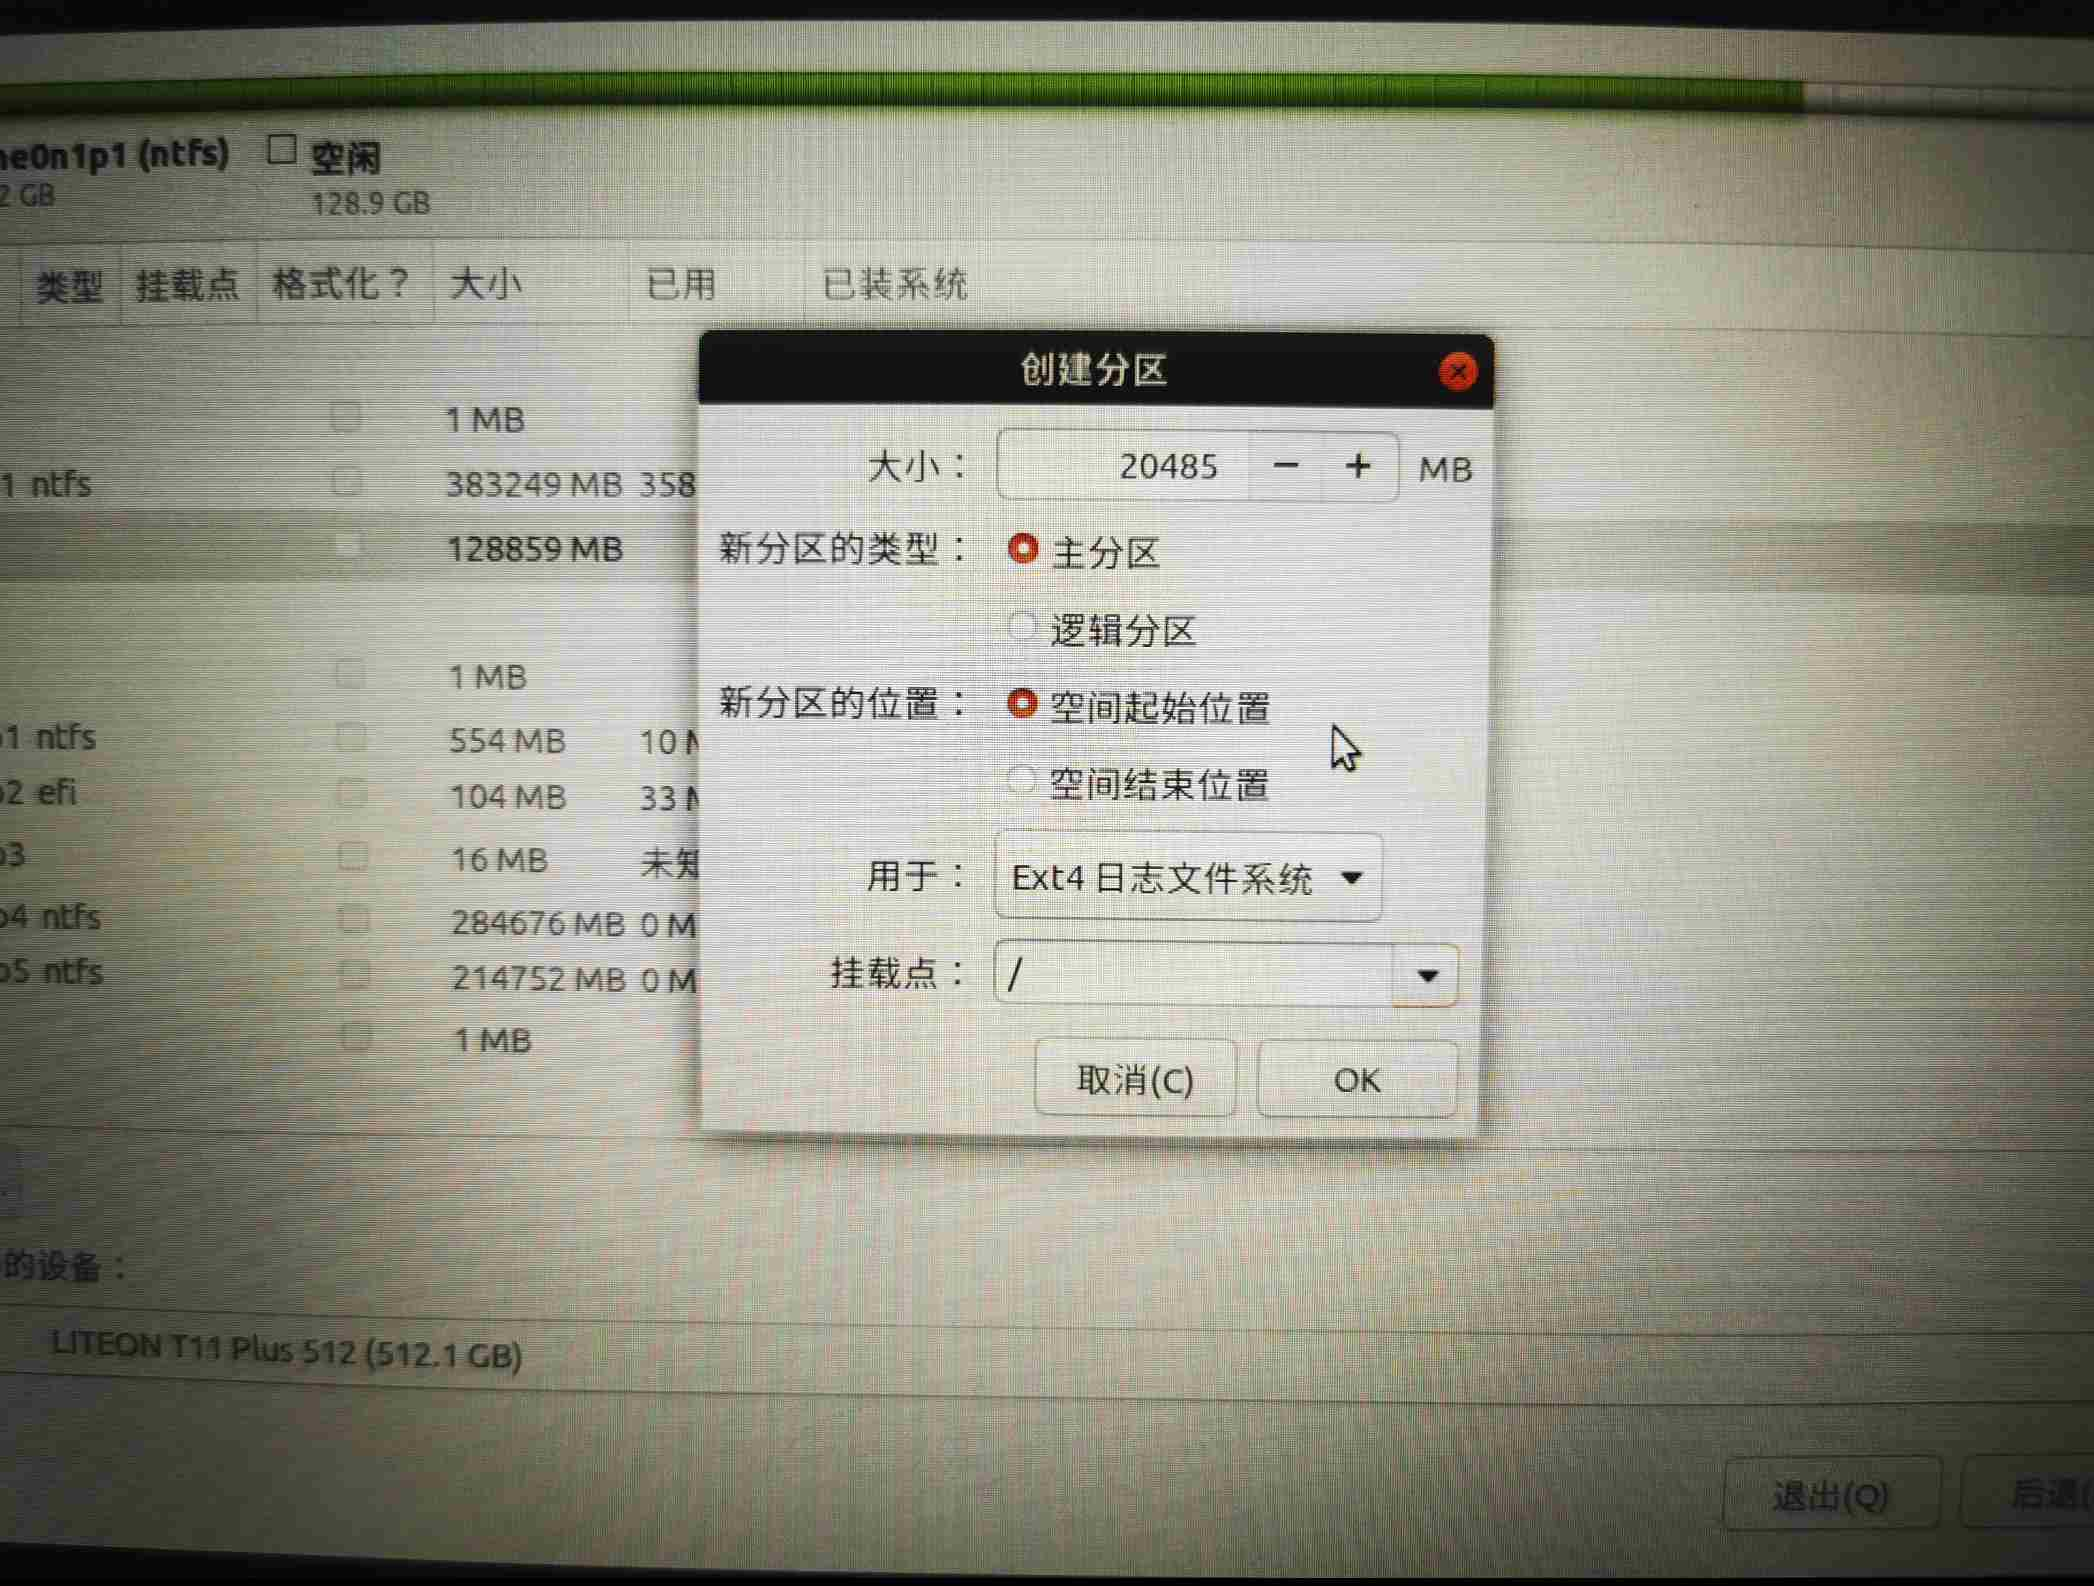
\includegraphics[width=0.45\linewidth]{png/system}
					}
					\hfill
					\subfigure[交换分区设置]{
						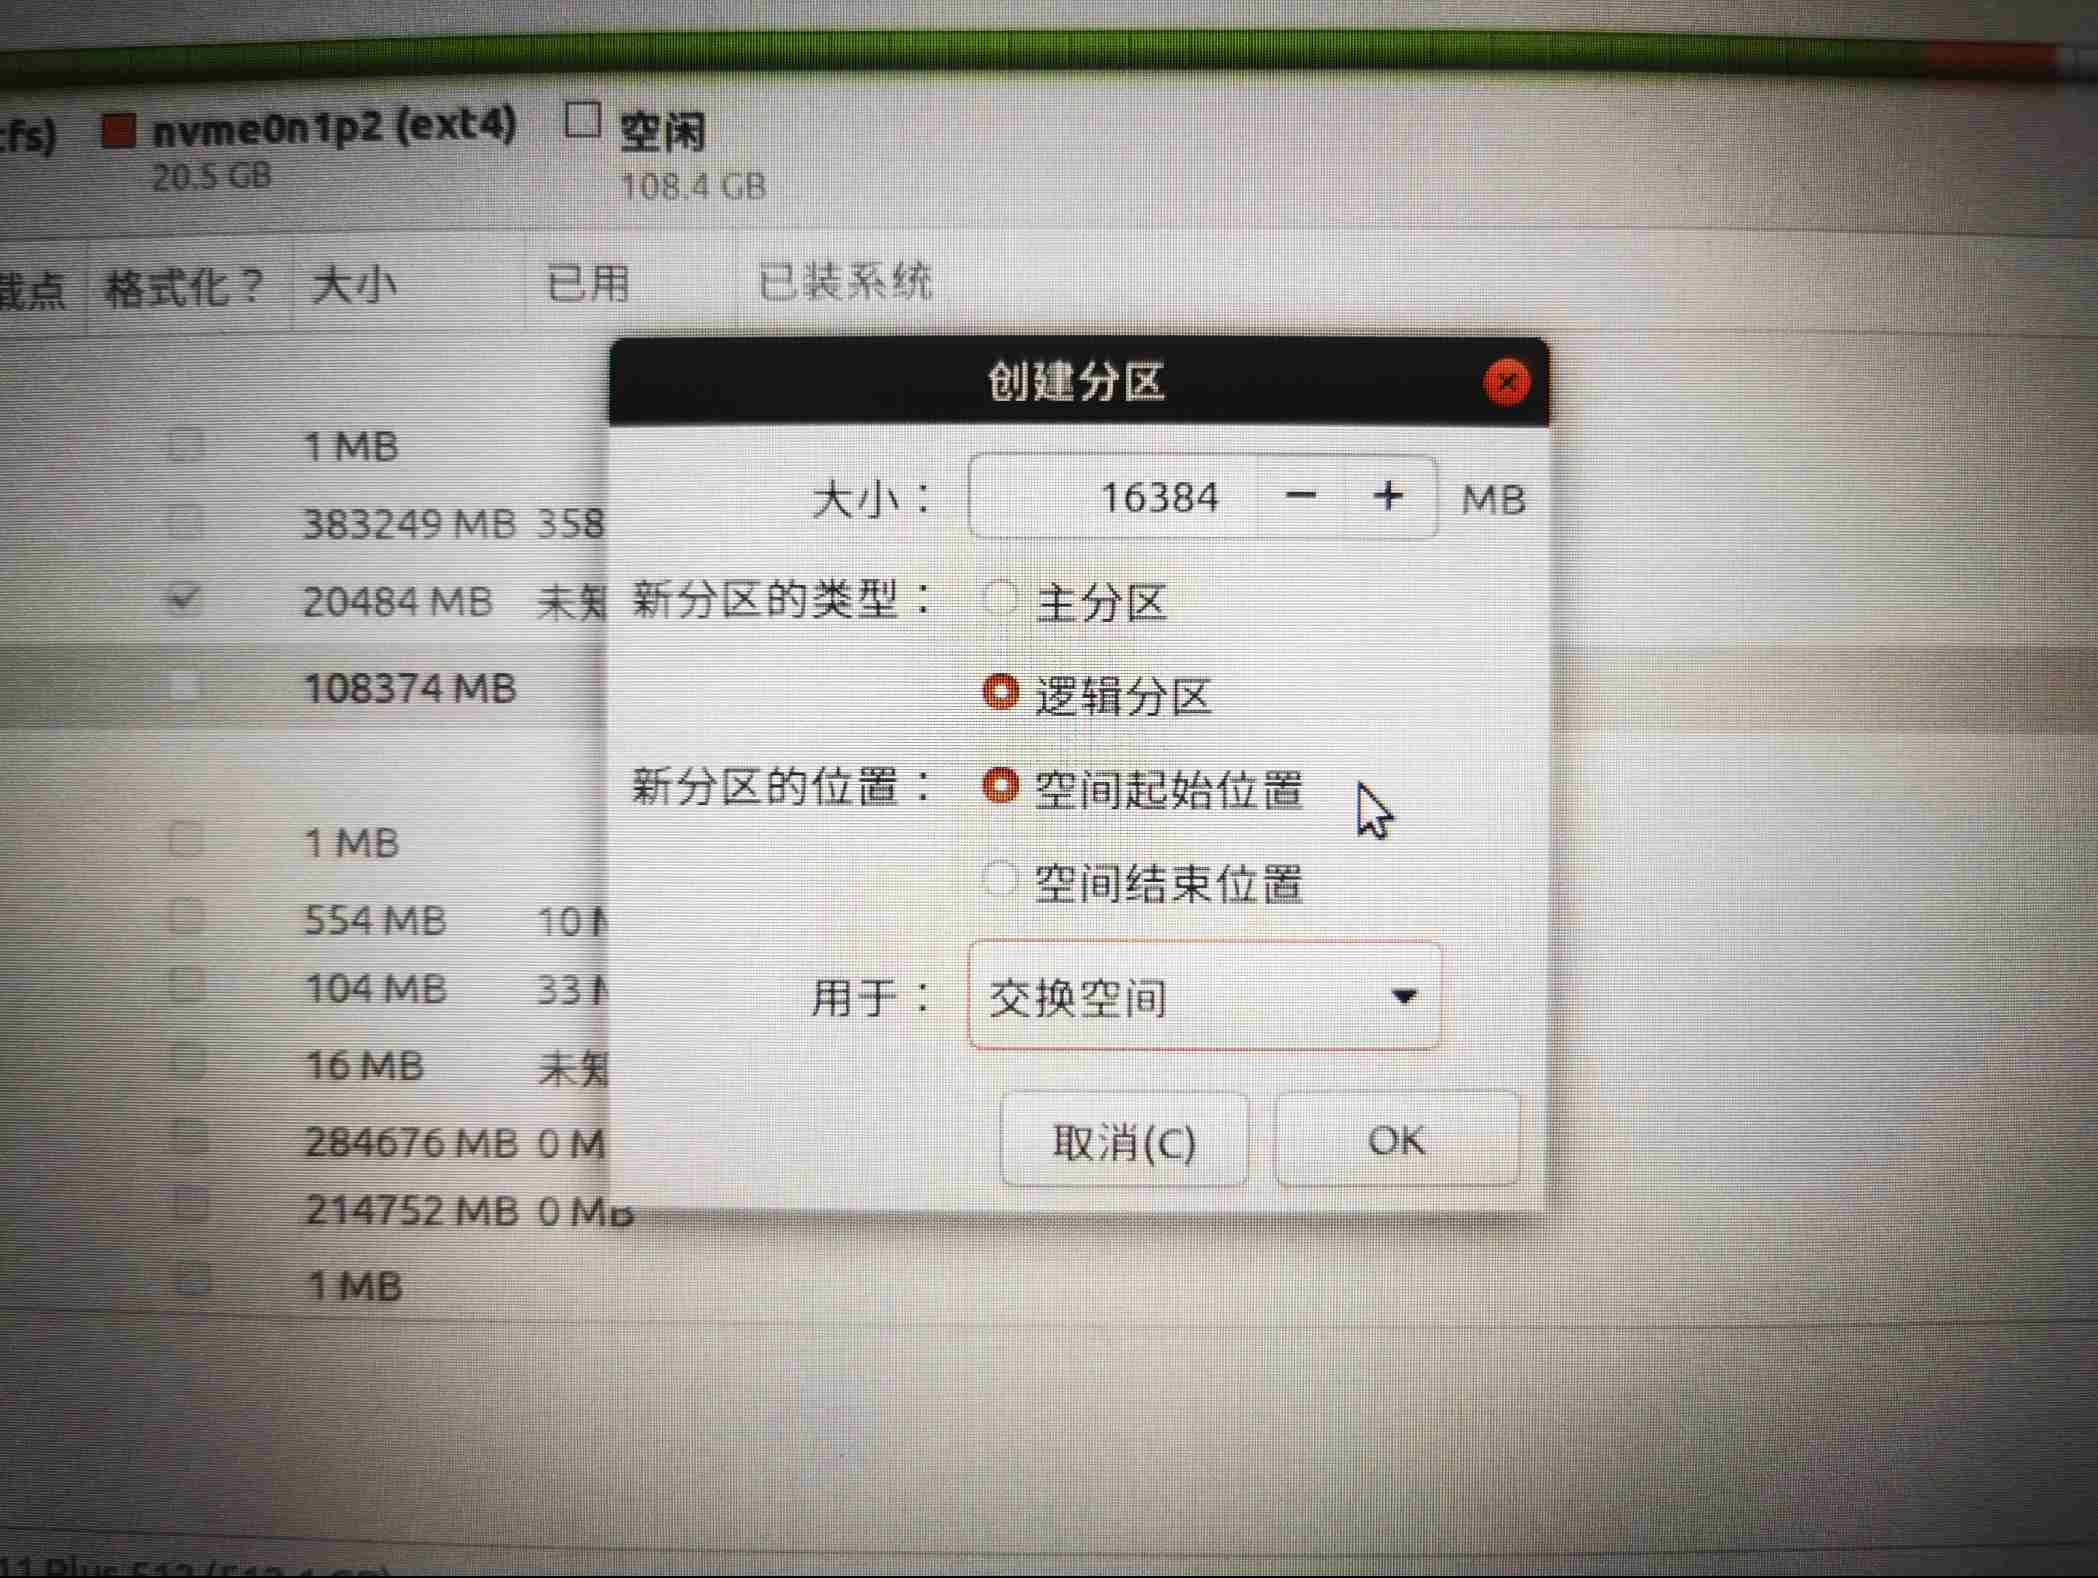
\includegraphics[width=0.45\linewidth]{png/swap}
					}
					\hfill
					\subfigure[boot分区设置]{
						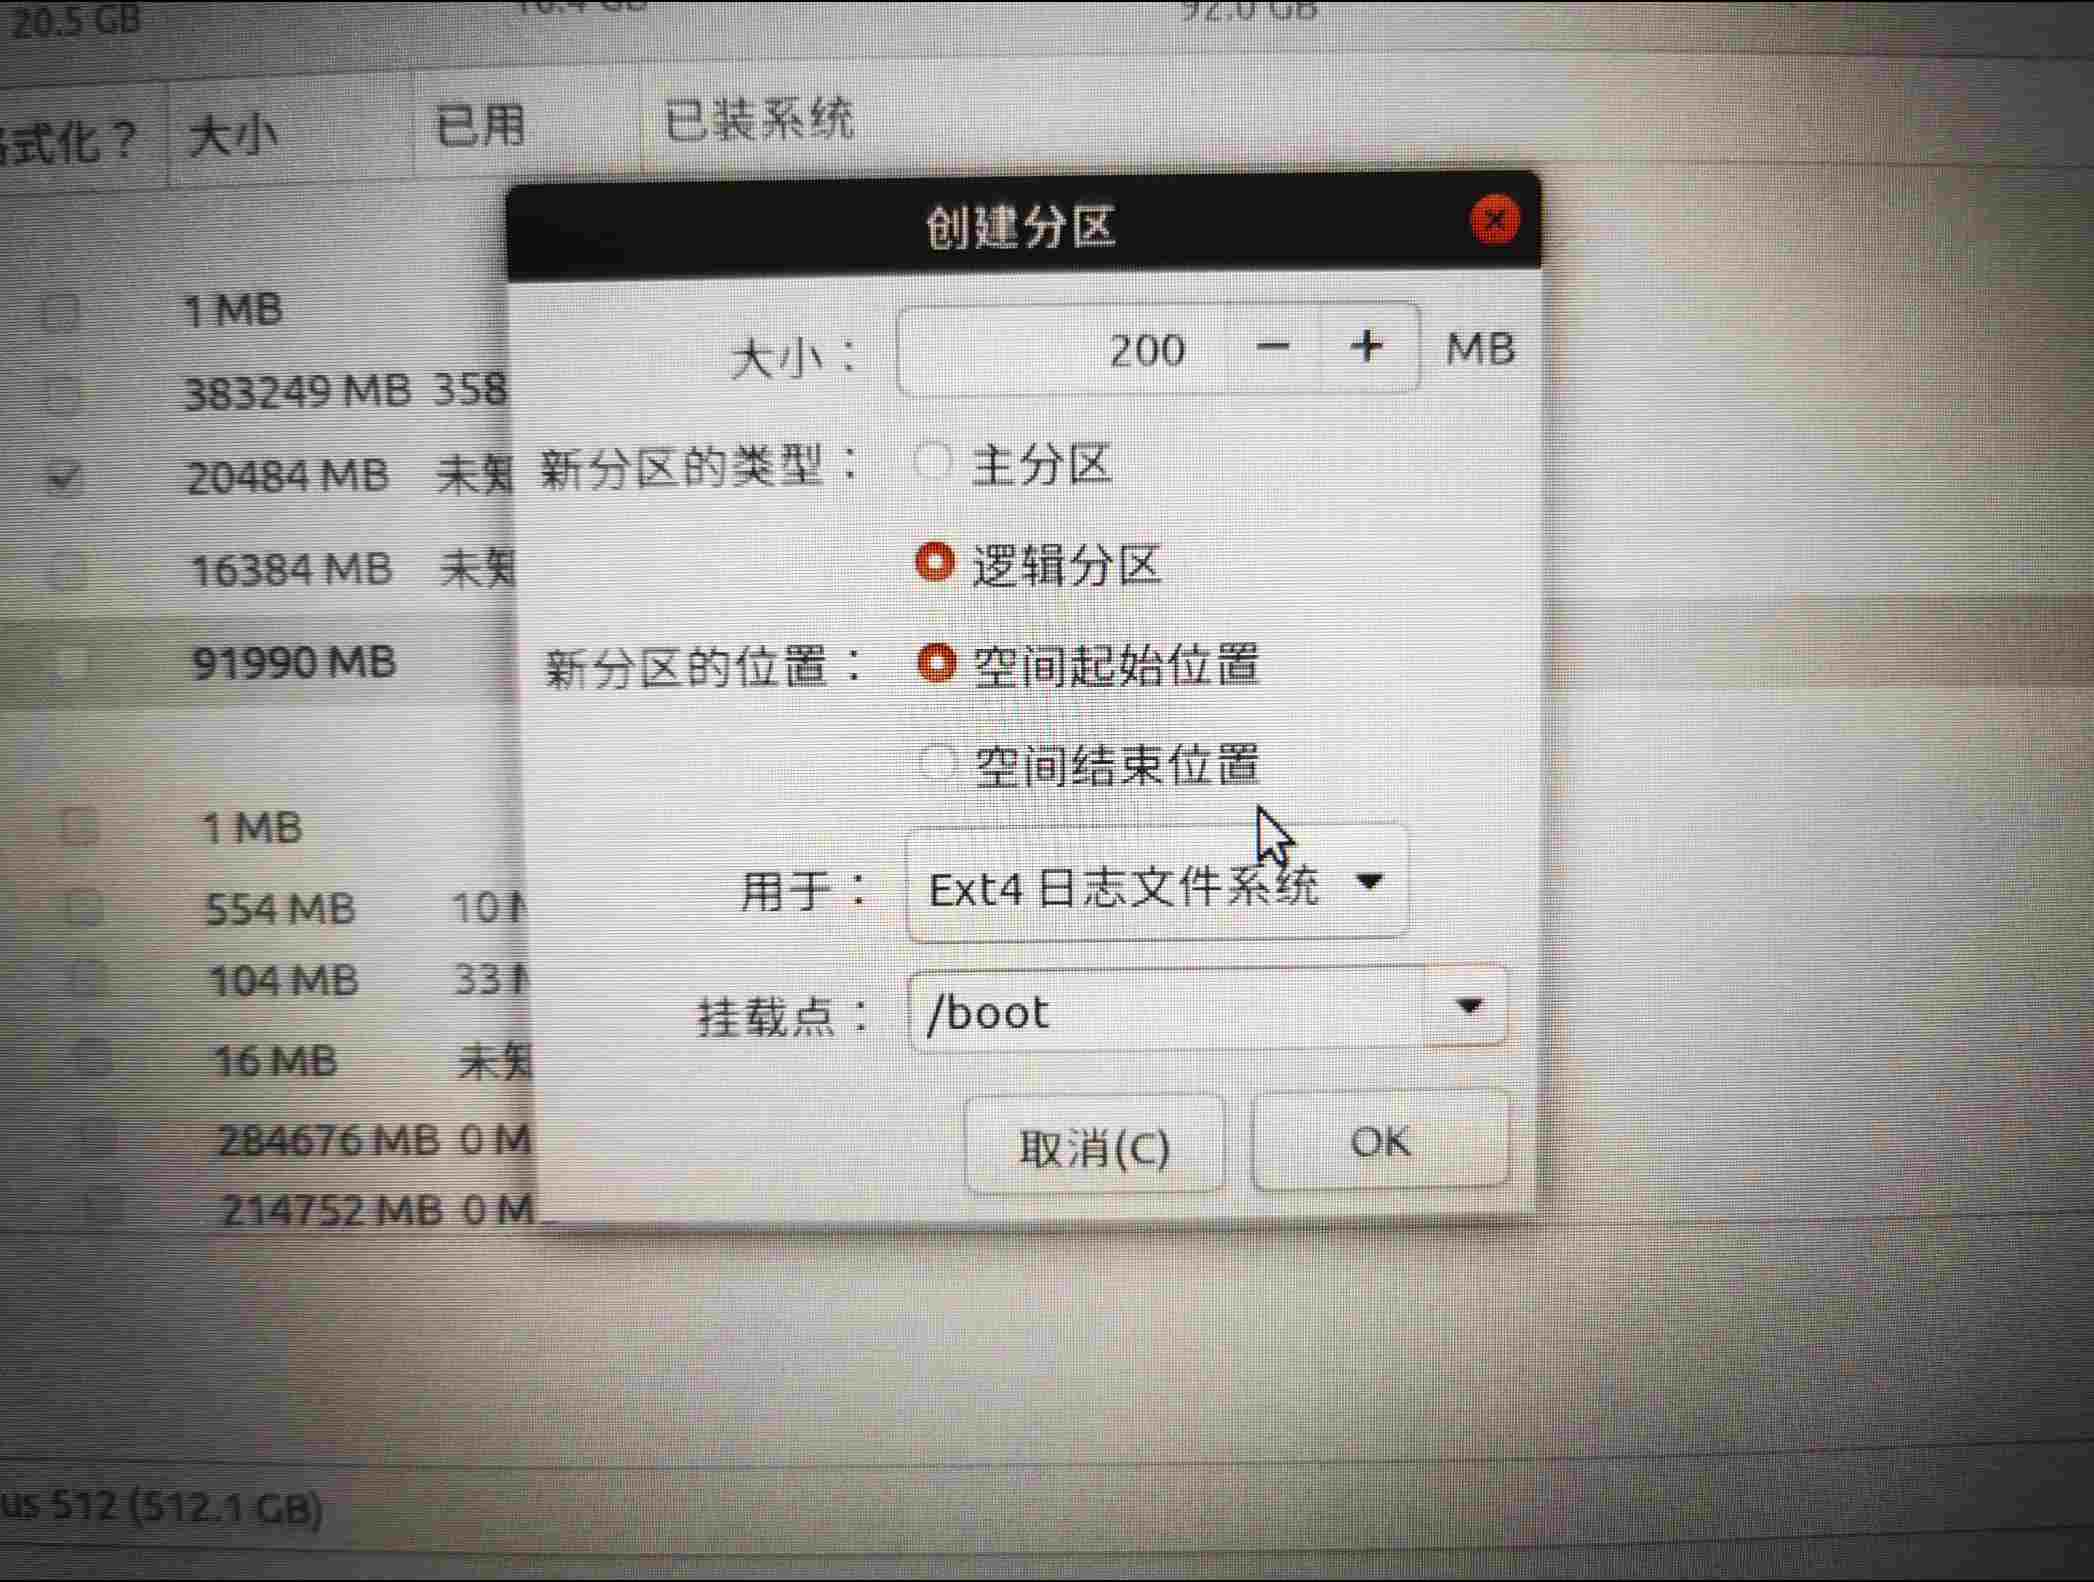
\includegraphics[width=0.45\linewidth]{png/boot}
					}
					\hfill
					\subfigure[用户分区设置]{
						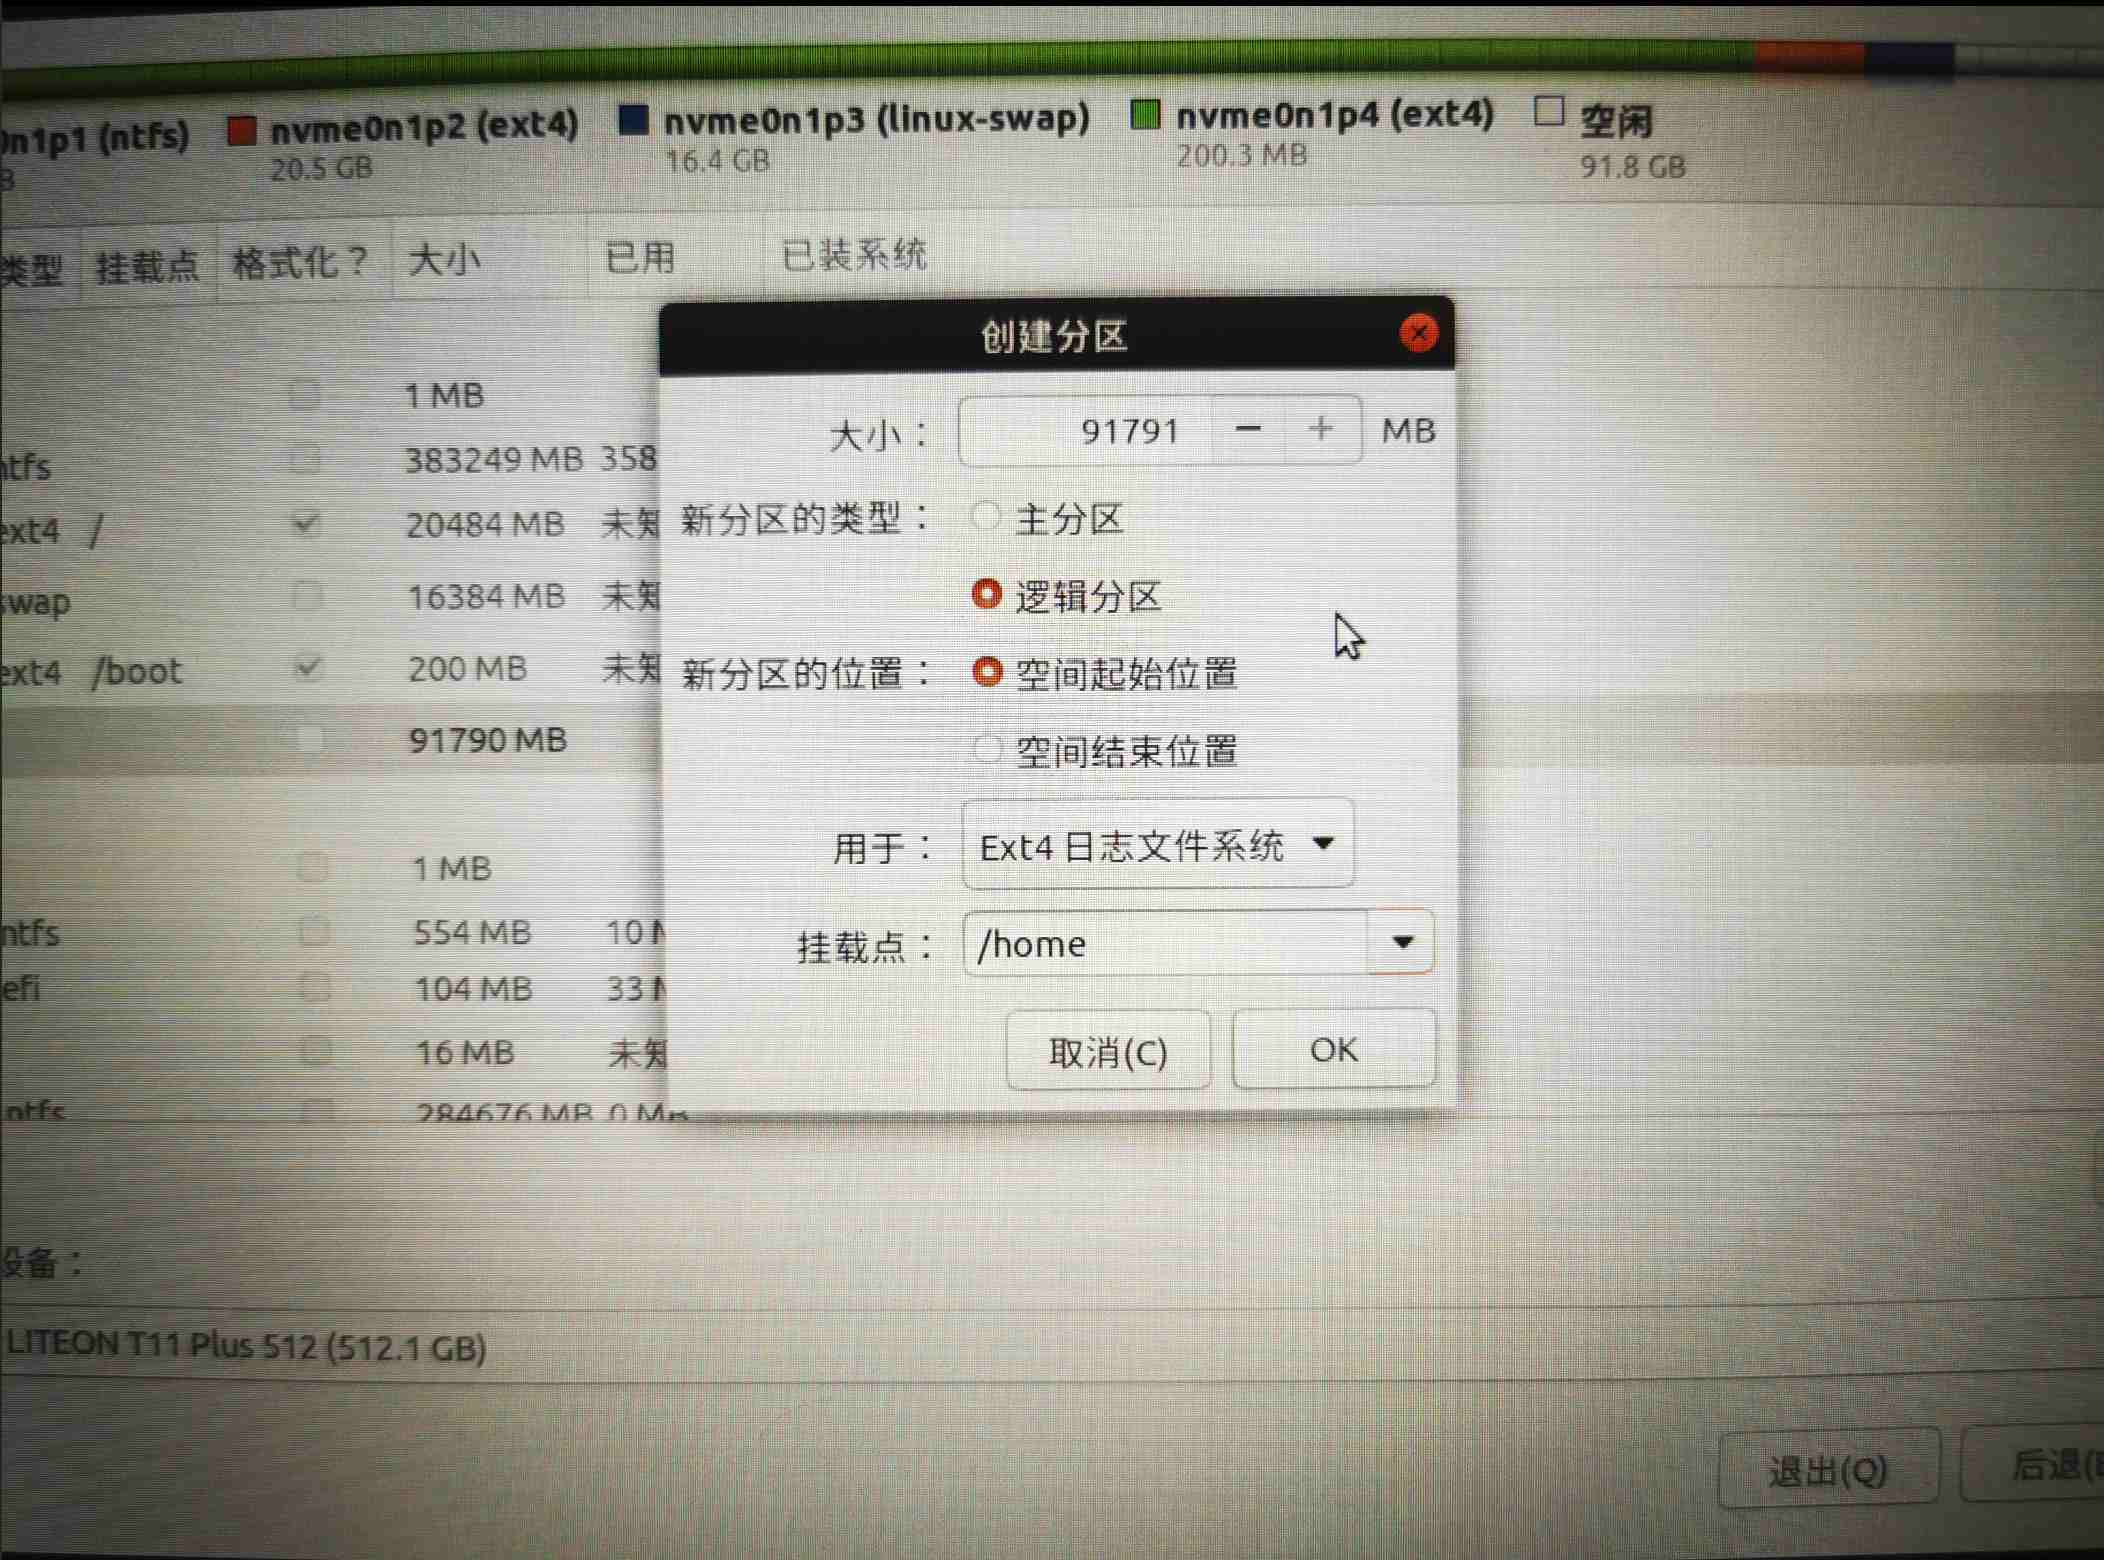
\includegraphics[width=0.45\linewidth]{png/user}
					}
				    \hfill
				    \subfigure[分区完成]{
				    	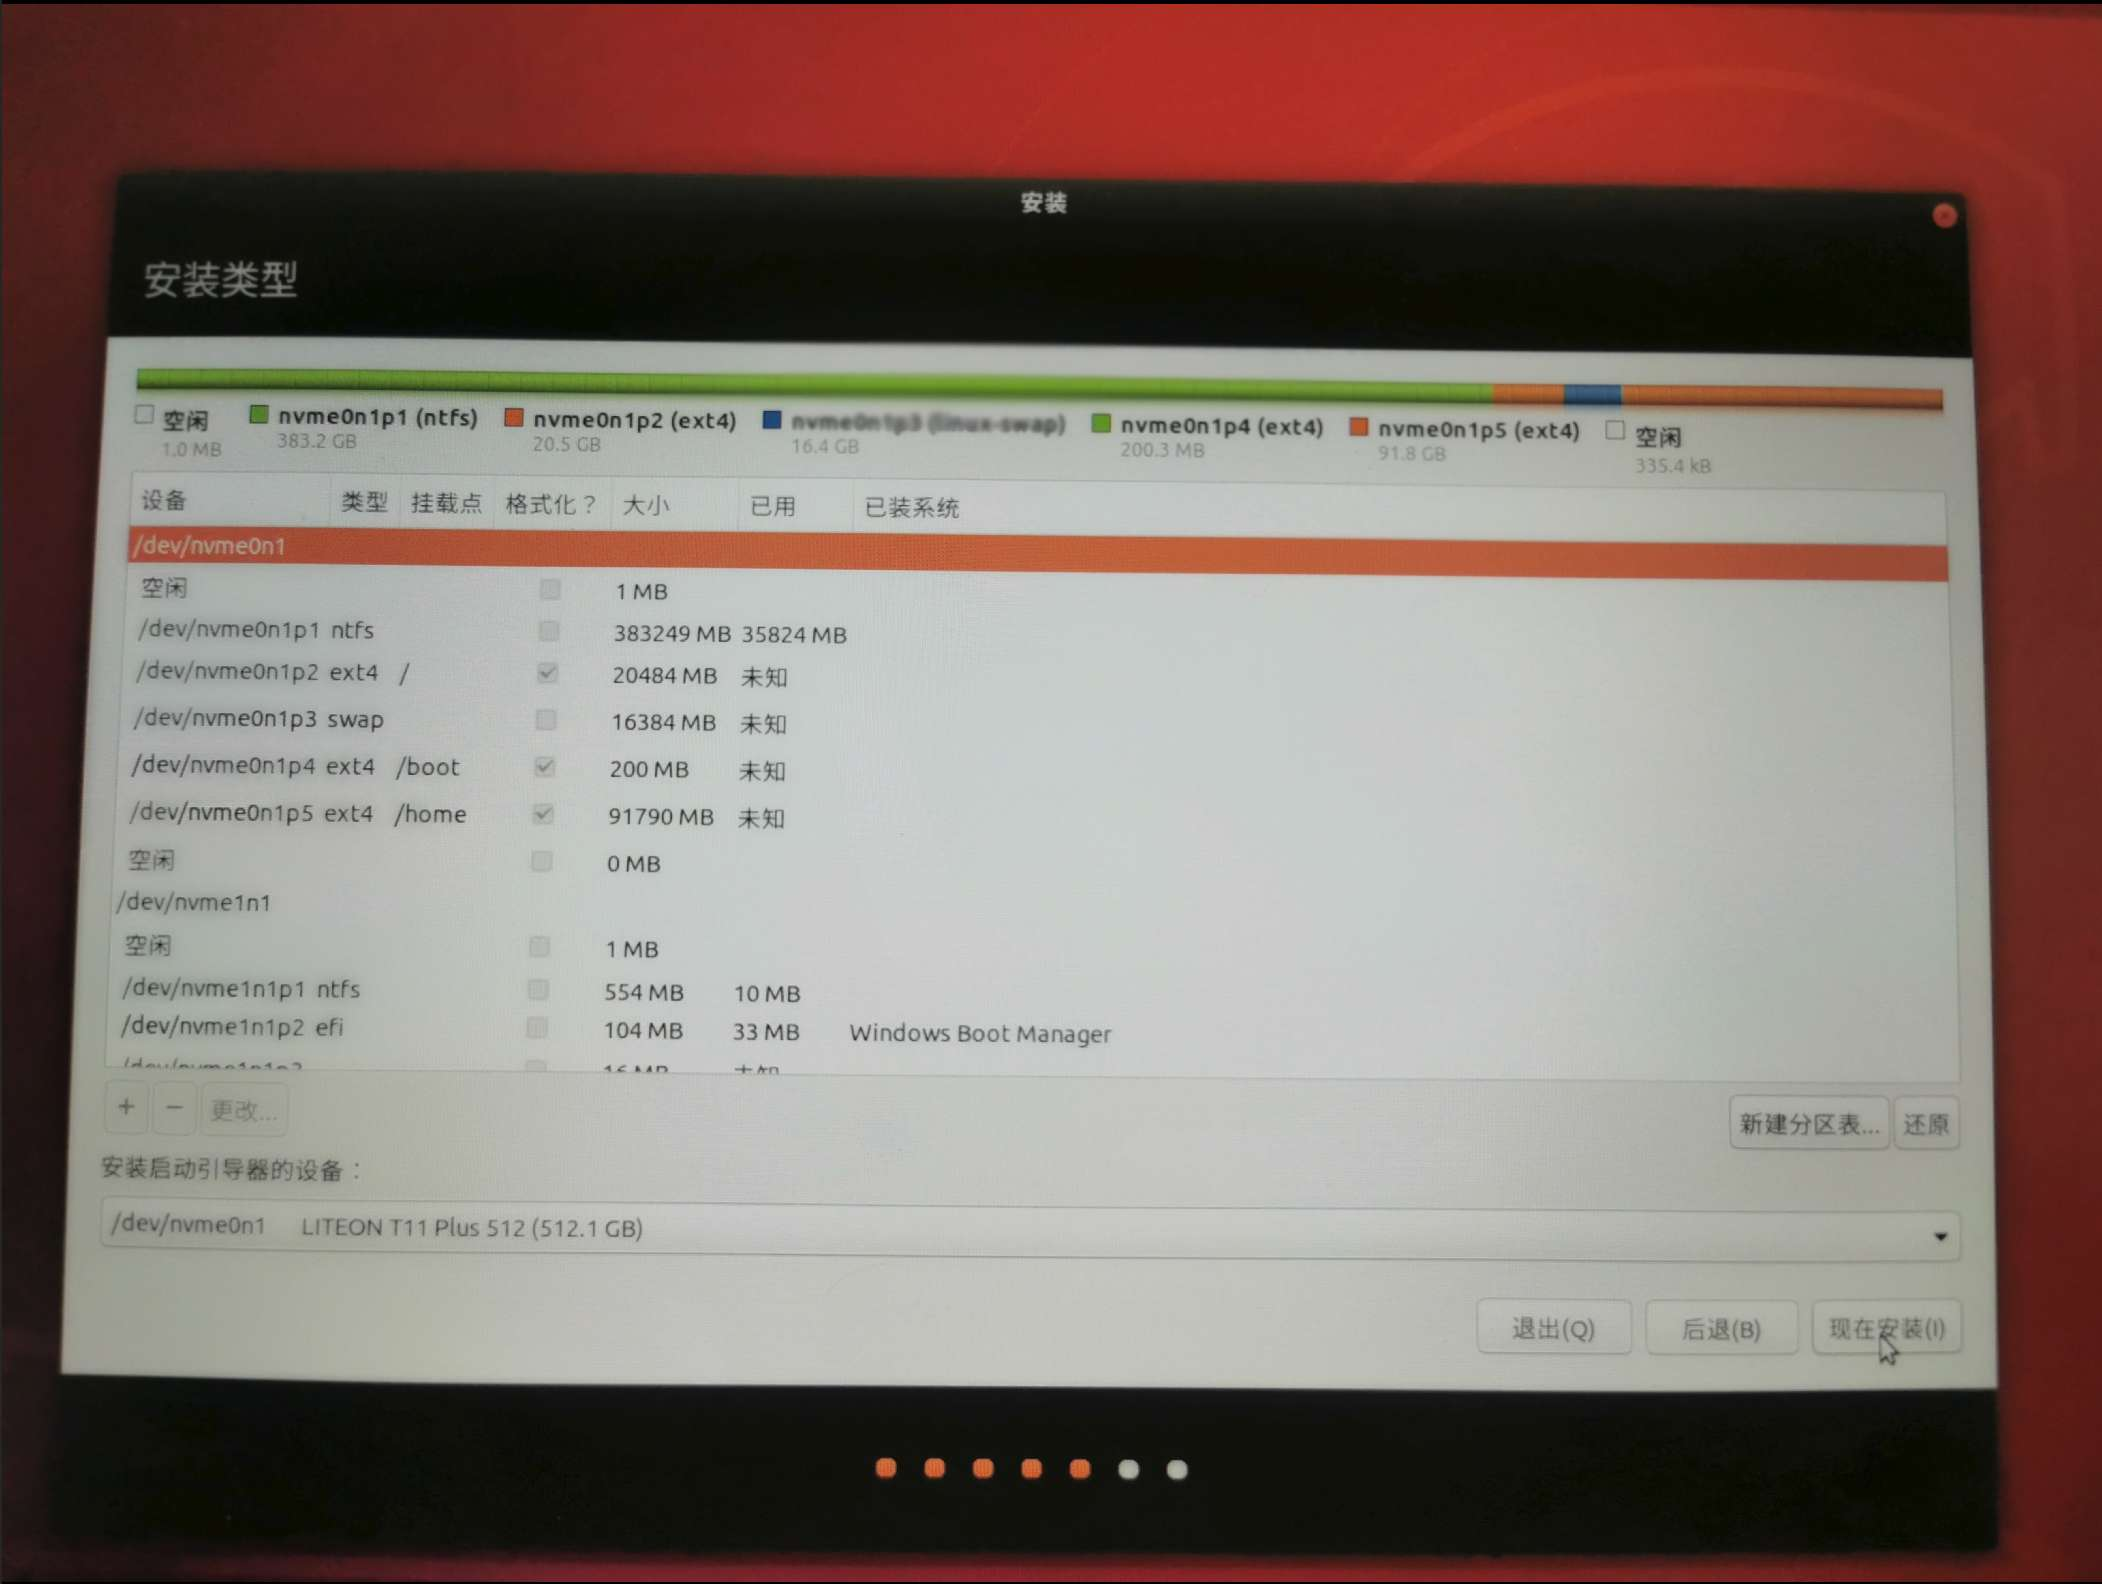
\includegraphics[width=0.8\linewidth]{png/allocated}
				    }
					\label{fig:setting}
				\end{figure}
			\item [II-c.] 分配之后的分区表会出现 4 个未知的新分区,然后点击继续安装。
				选择时区和用户名密码,自行设置后等待安装完成。
		\end{itemize}
\end{itemize}



\subsection{Ubuntu 上的软件安装}

如果你已经成功的安装了 Ubuntu 系统,
那么接下来你应该做的是在这个系统里面安装一些你需要的软件来丰富它。
在 Ubuntu 中安装软件和 Windows 系统中双击 exe 文件安装软件的方式有很大的不同,
在 Ubuntu 中主要有以下两种安装的方式。

\textbf{命令行安装:} Ubuntu 上软件安装的最常见方式是直接在终端(Ctrl+Alt+T)输入相应安装命令。
常见的有
\begin{itemize}
	\item apt-get安装;
	\item dpkg安装;
	\item 编译安装。
\end{itemize}

apt-get 安装是最常见的安装方式,其基本的安装命令为
\begin{verbatim}
sudo apt-get install package  // package 为需要安装的软件。
\end{verbatim}

区别于 apt 安装方式,dpkg 只是用来安装本地软件包(deb包),但不解决模块的依赖关系。
而 apt 是从网络服务器下载并安装软件包的,它会解决依赖关系。
其基本的安装命令为
\begin{verbatim}
dpkg -i package.deb。
\end{verbatim}
由于 dpkg 的安装方式不会解决依赖的问题,所以经常会出现安装过程中依赖未安装的情况,
可以通过
\begin{verbatim}
sudo apt install -f	
\end{verbatim}
来修复依赖。

对于一些需要自己下载源代码编译安装的情况,
首先解压进入文件夹,一般都会有 README 或 install 文件指导你安装的过程,
通常过程为
\begin{verbatim}
./configure
make
sudo make install。
\end{verbatim}

\textbf{软件包管理器安装:}软件包管理器是 Ubuntu 的包管理工具 apt 的图形化前端。
它结合了图形界面的简单操作和 apt-get 命令行工具的强大功能。
它能跟踪所有已安装的软件、自动化进行安装和删除应用程序、
以及确保所有软件都保持更新以获得最新的增强功能和错误修复。
我们所需要做的仅仅是决定我们想安装哪个应用程序,
然后使用软件包管理器来告诉 Ubuntu 去安装它们。
常见的有
\begin{itemize}
	\item Ubuntu 软件中心;
	\item 新立得软件包管理器。
\end{itemize}

Ubuntu 软件中心是最容易使用的,它能让你安装和卸载许多流行软件包。
你可以简单地搜索如 'emacs' 这种关键字来搜索您想安装的软件包,或浏览给出的分类,
选择应用程序,将进入应用程序介绍页面,此页面将给出应用程序截图和简要介绍,
点击下方的“安装”按钮,获得授权后即开始安装软件。
\begin{figure}[htbp]
	\centering
	\subfigure[Ubuntu 软件中心界面]{
		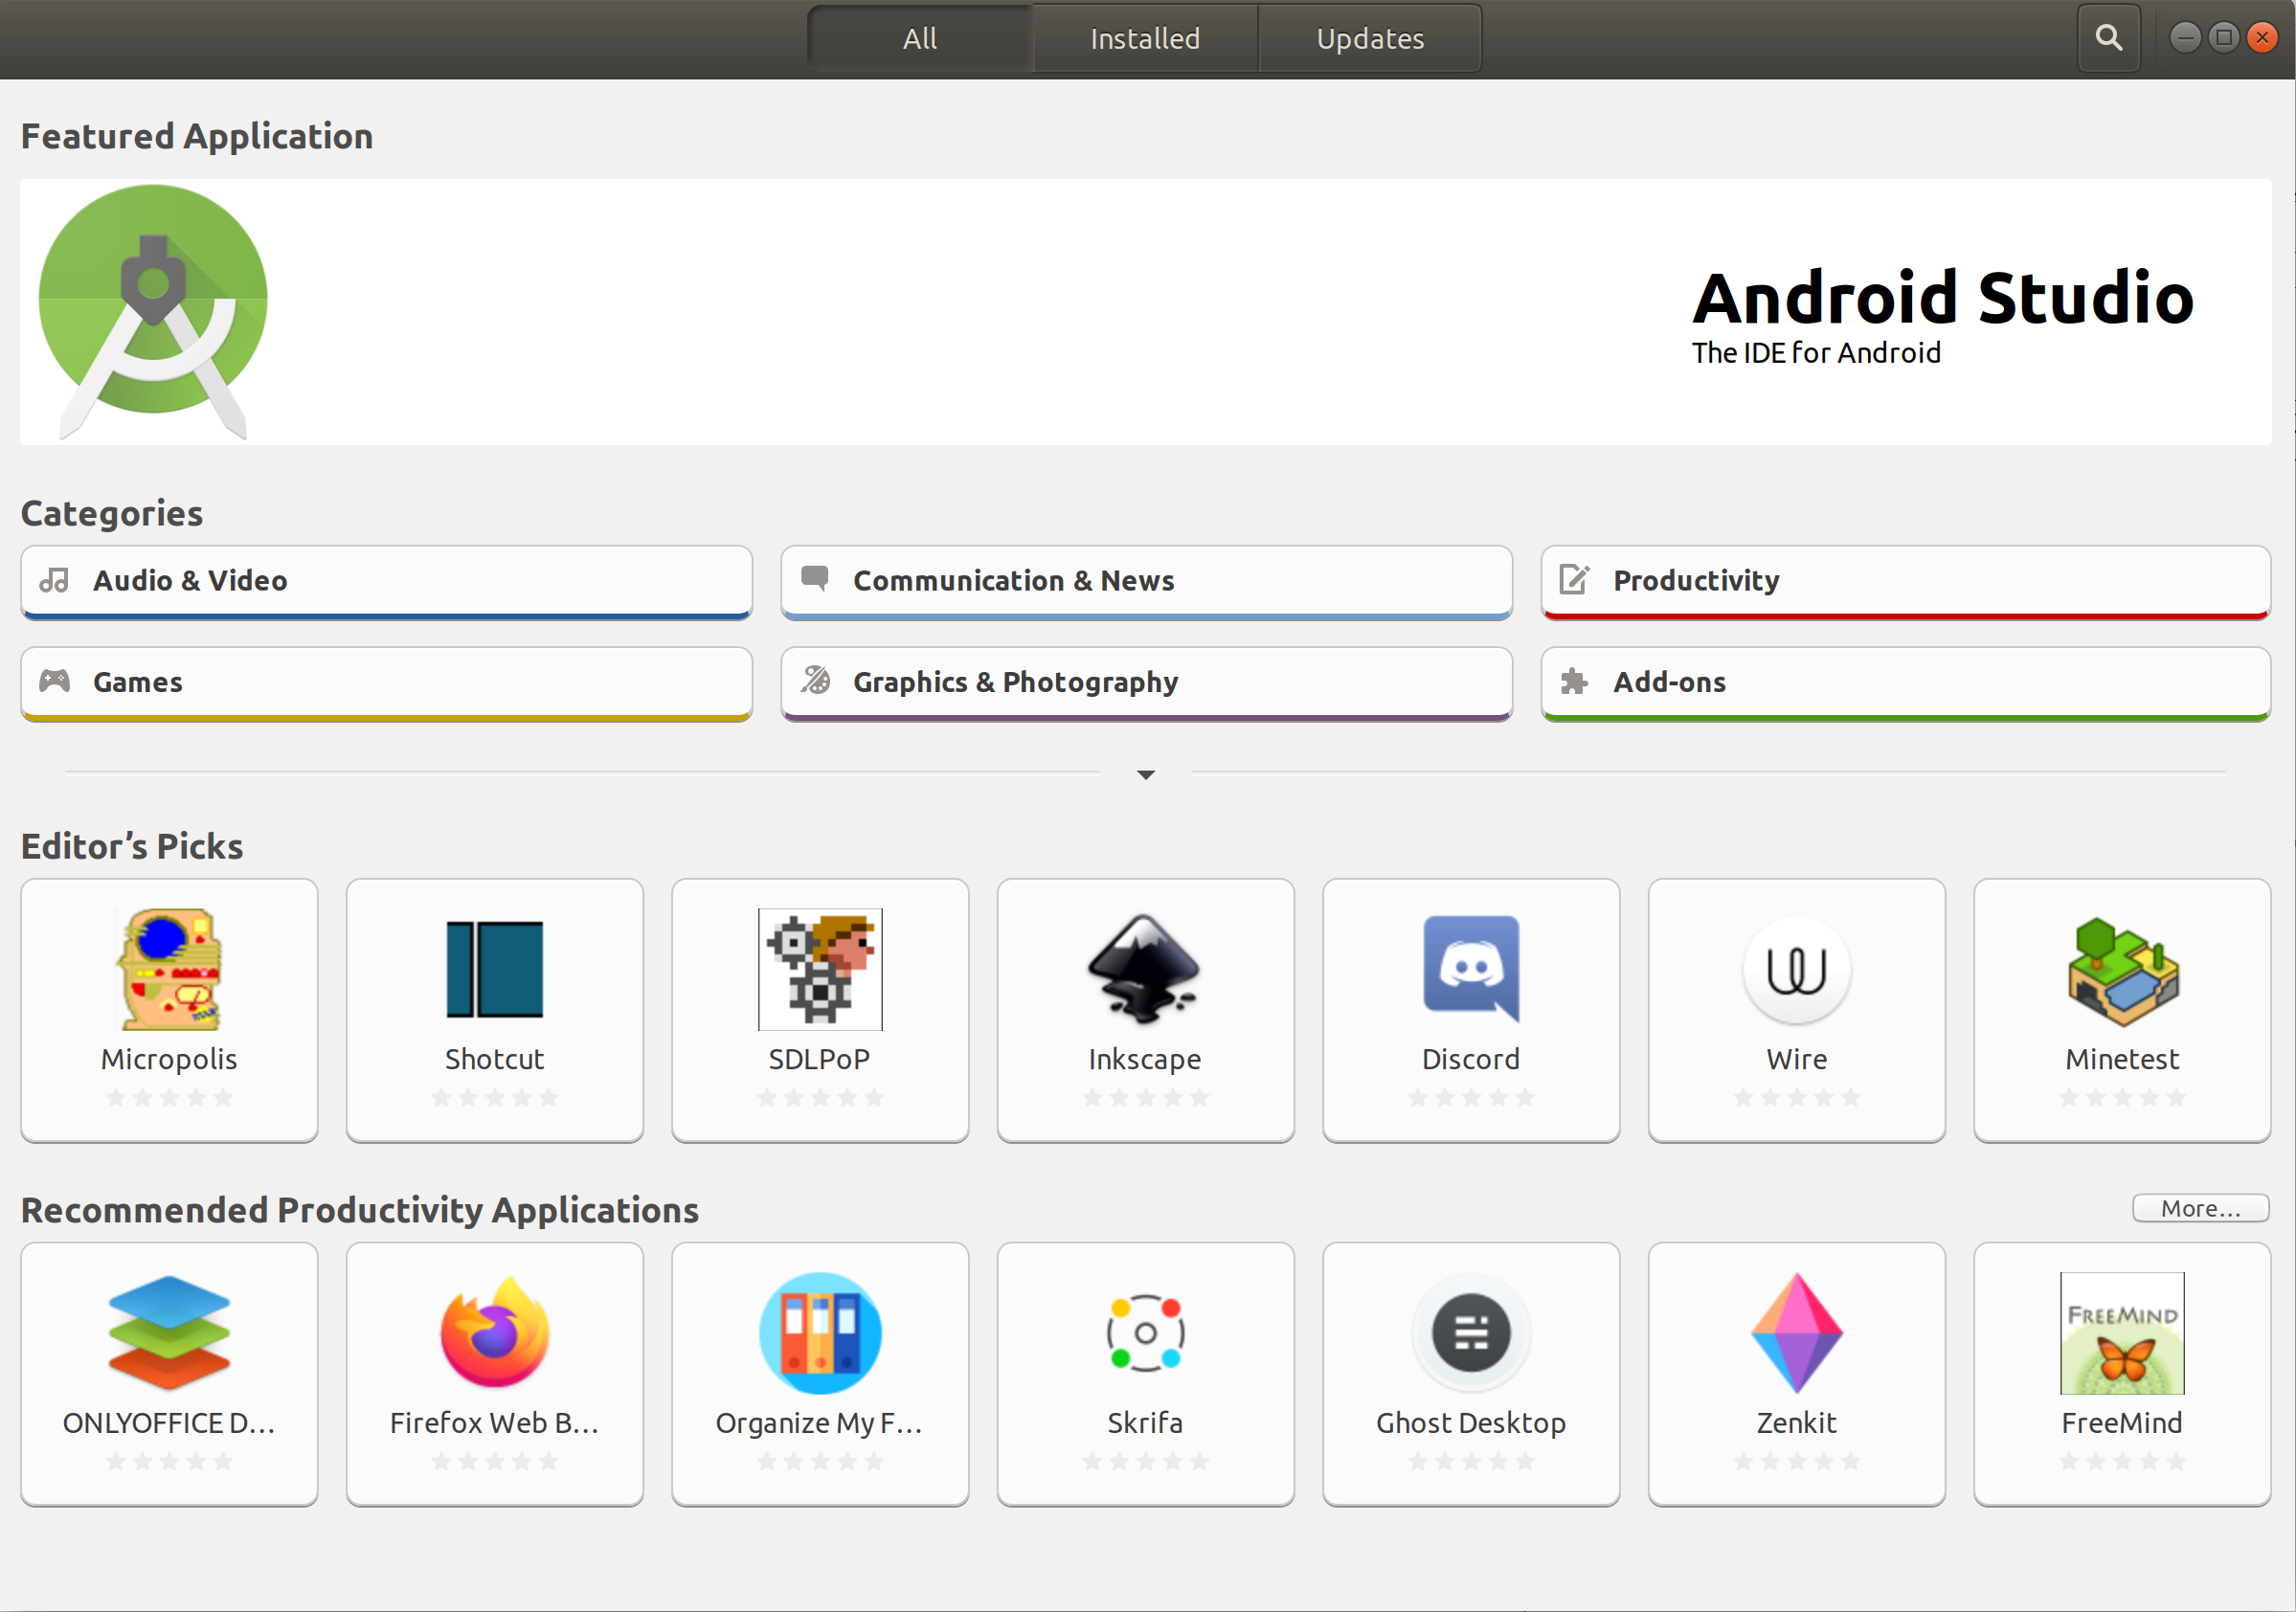
\includegraphics[width=0.45\linewidth]{png/ubuntuSoftware}
	}
	\hfill
	\subfigure[使用 Ubuntu 软件中心安装软件]{
		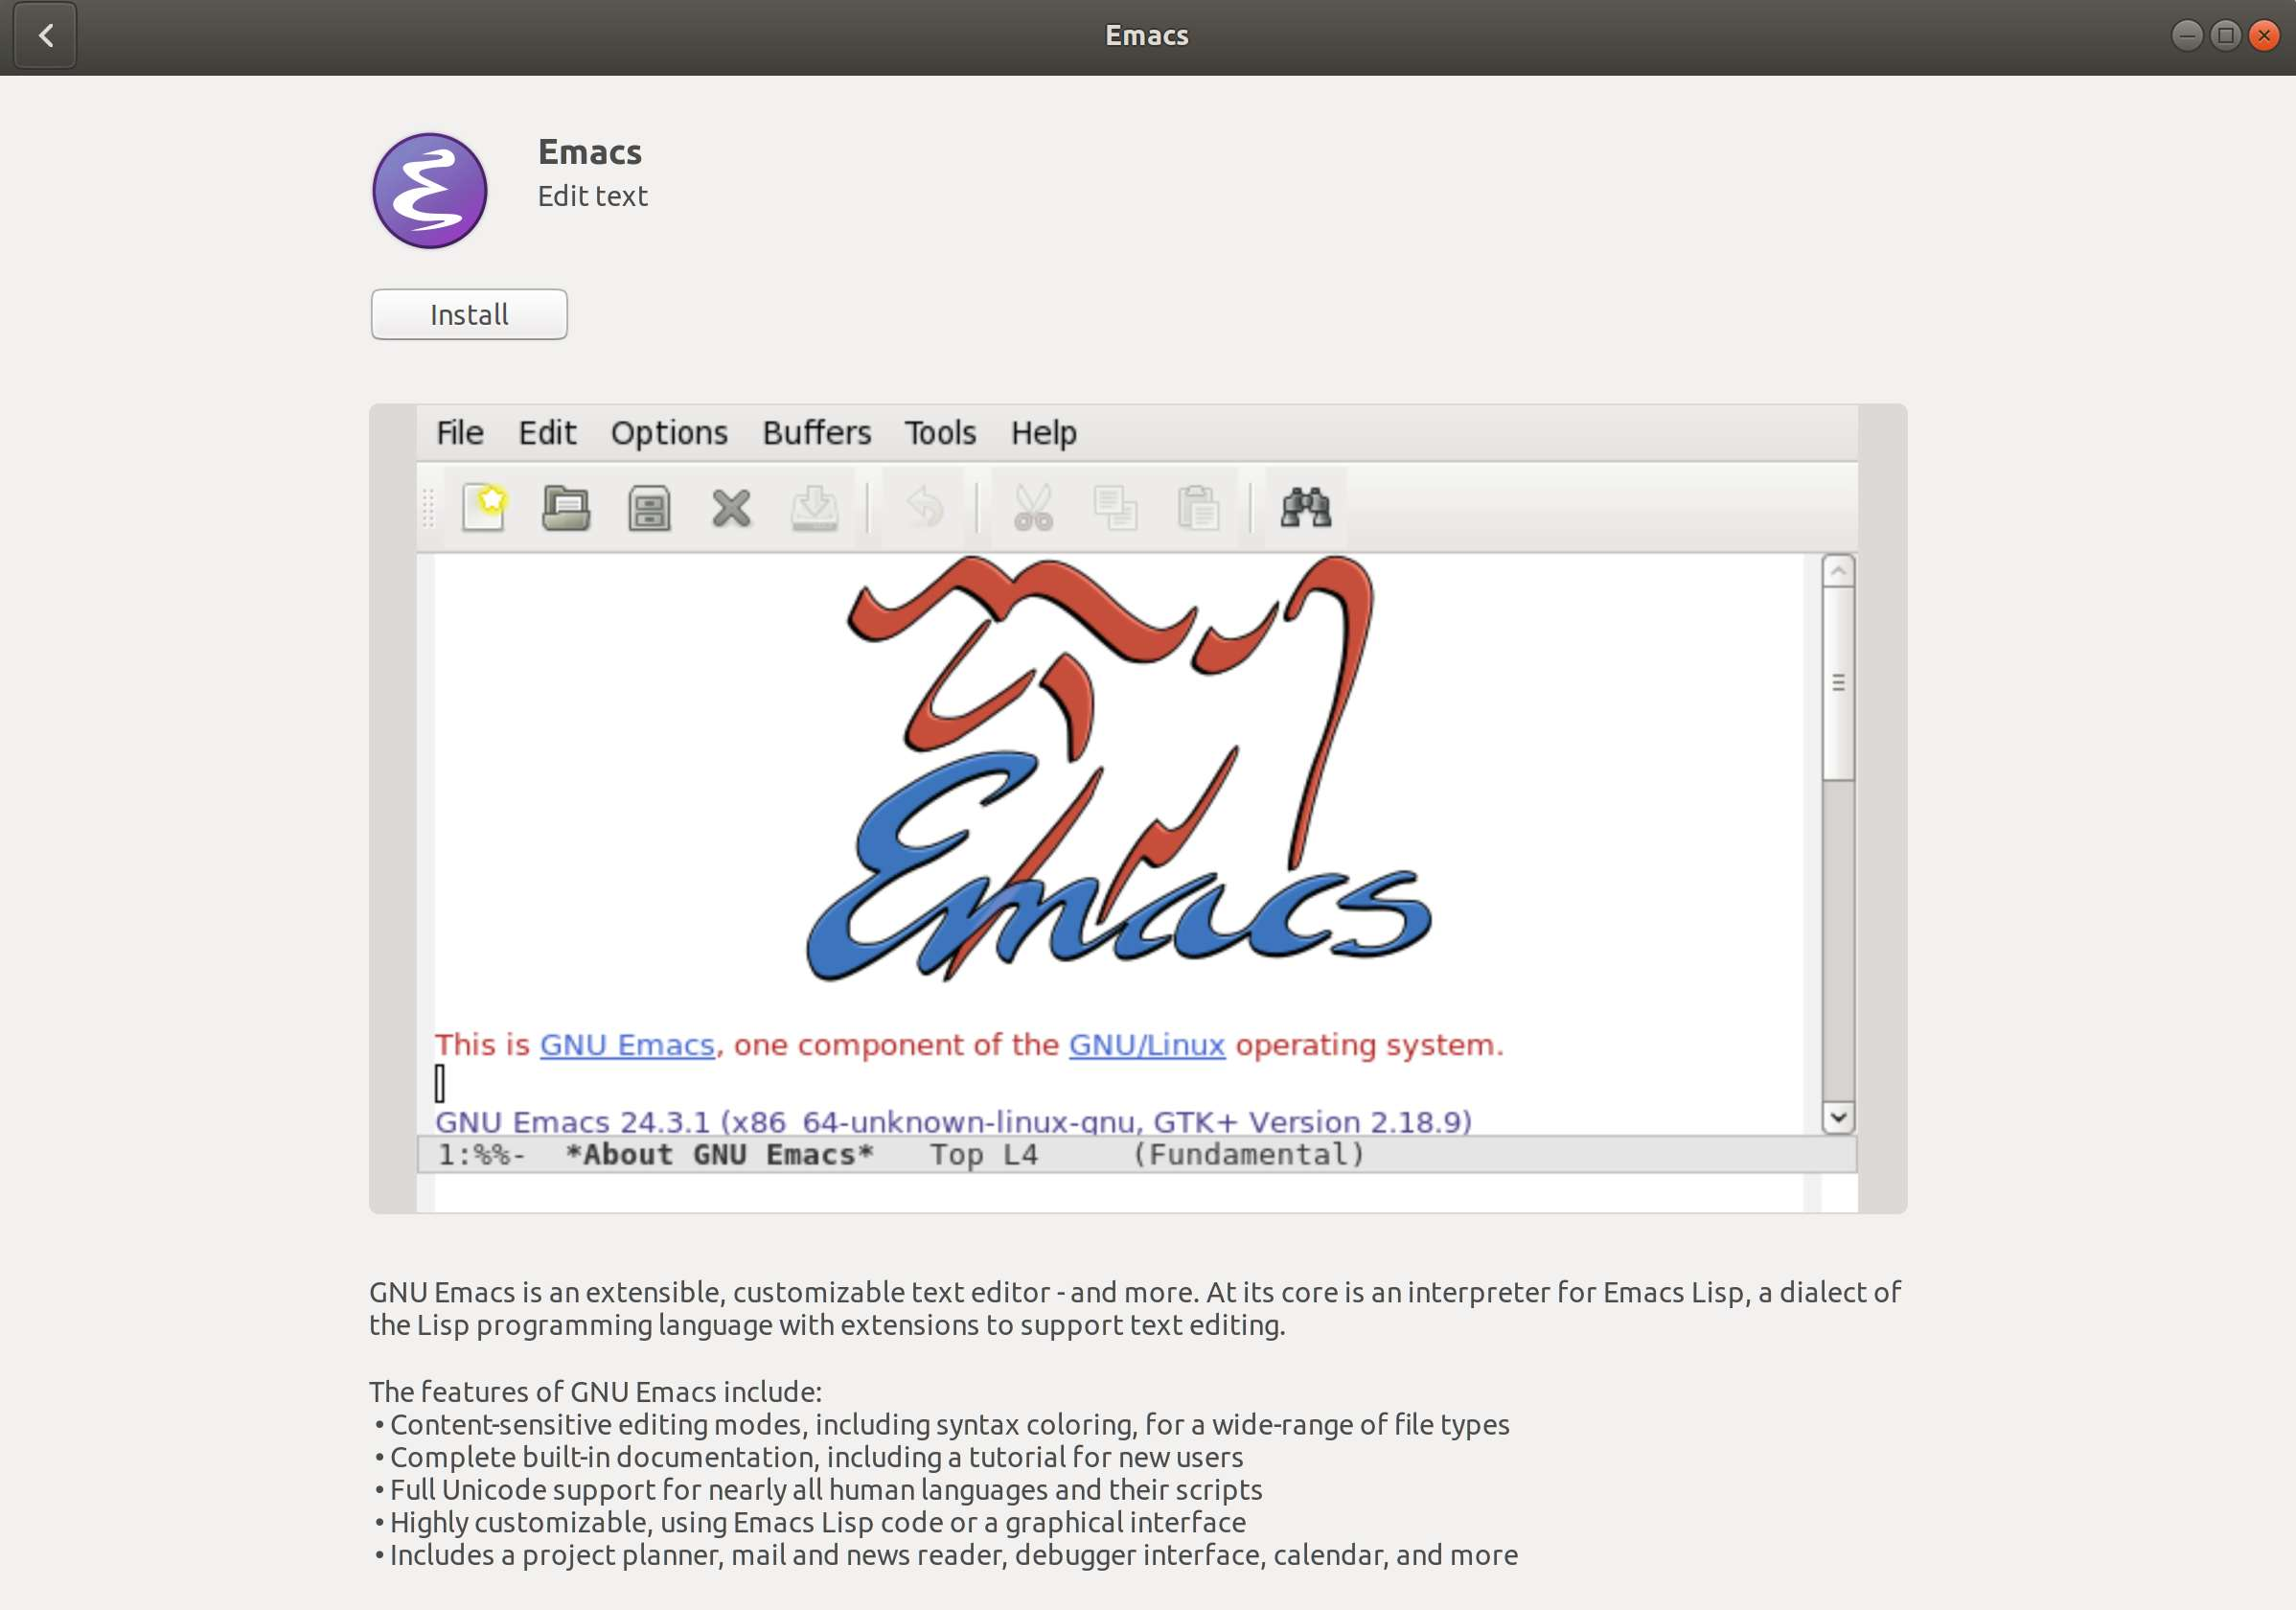
\includegraphics[width=0.45\linewidth]{png/emacsInstall}
	}
	\label{fig:Software}
\end{figure}

使用 Ubuntu 软件中心无法让您安装和删除某些更高级的软件包,
比如 Apache 网络服务、PHP 编程语言或 Scribus。这时,就得用新立得软件包管理器。
如果你的 Ubuntu 系统没有默认安装新立得软件包管理器(Synaptic Package Manager),
使用前需要安装它,基本命令为
\begin{verbatim}
sudo apt-get install synaptic。
\end{verbatim}

在新立得软件包管理器对话框中,你可以选择你需要的软件包。
左侧面板列出的是分类,右侧面板列出的是软件包。
点击搜索,将弹出查找对话框。在搜索字段中输入软件包的名称并点击搜索。
然后选择查找到的软件包,标记以便安装复选框来安装软件包。
如果你选择删除或安装的软件包依赖于其他软件包,你将得到依赖关系的通知。
点击标记以继续作出更改。
最后确认你想要进行标记的更改,点击应用即可自动安装。
\begin{figure}[htbp]
	\centering
	\subfigure[新立得软件包管理器界面]{
		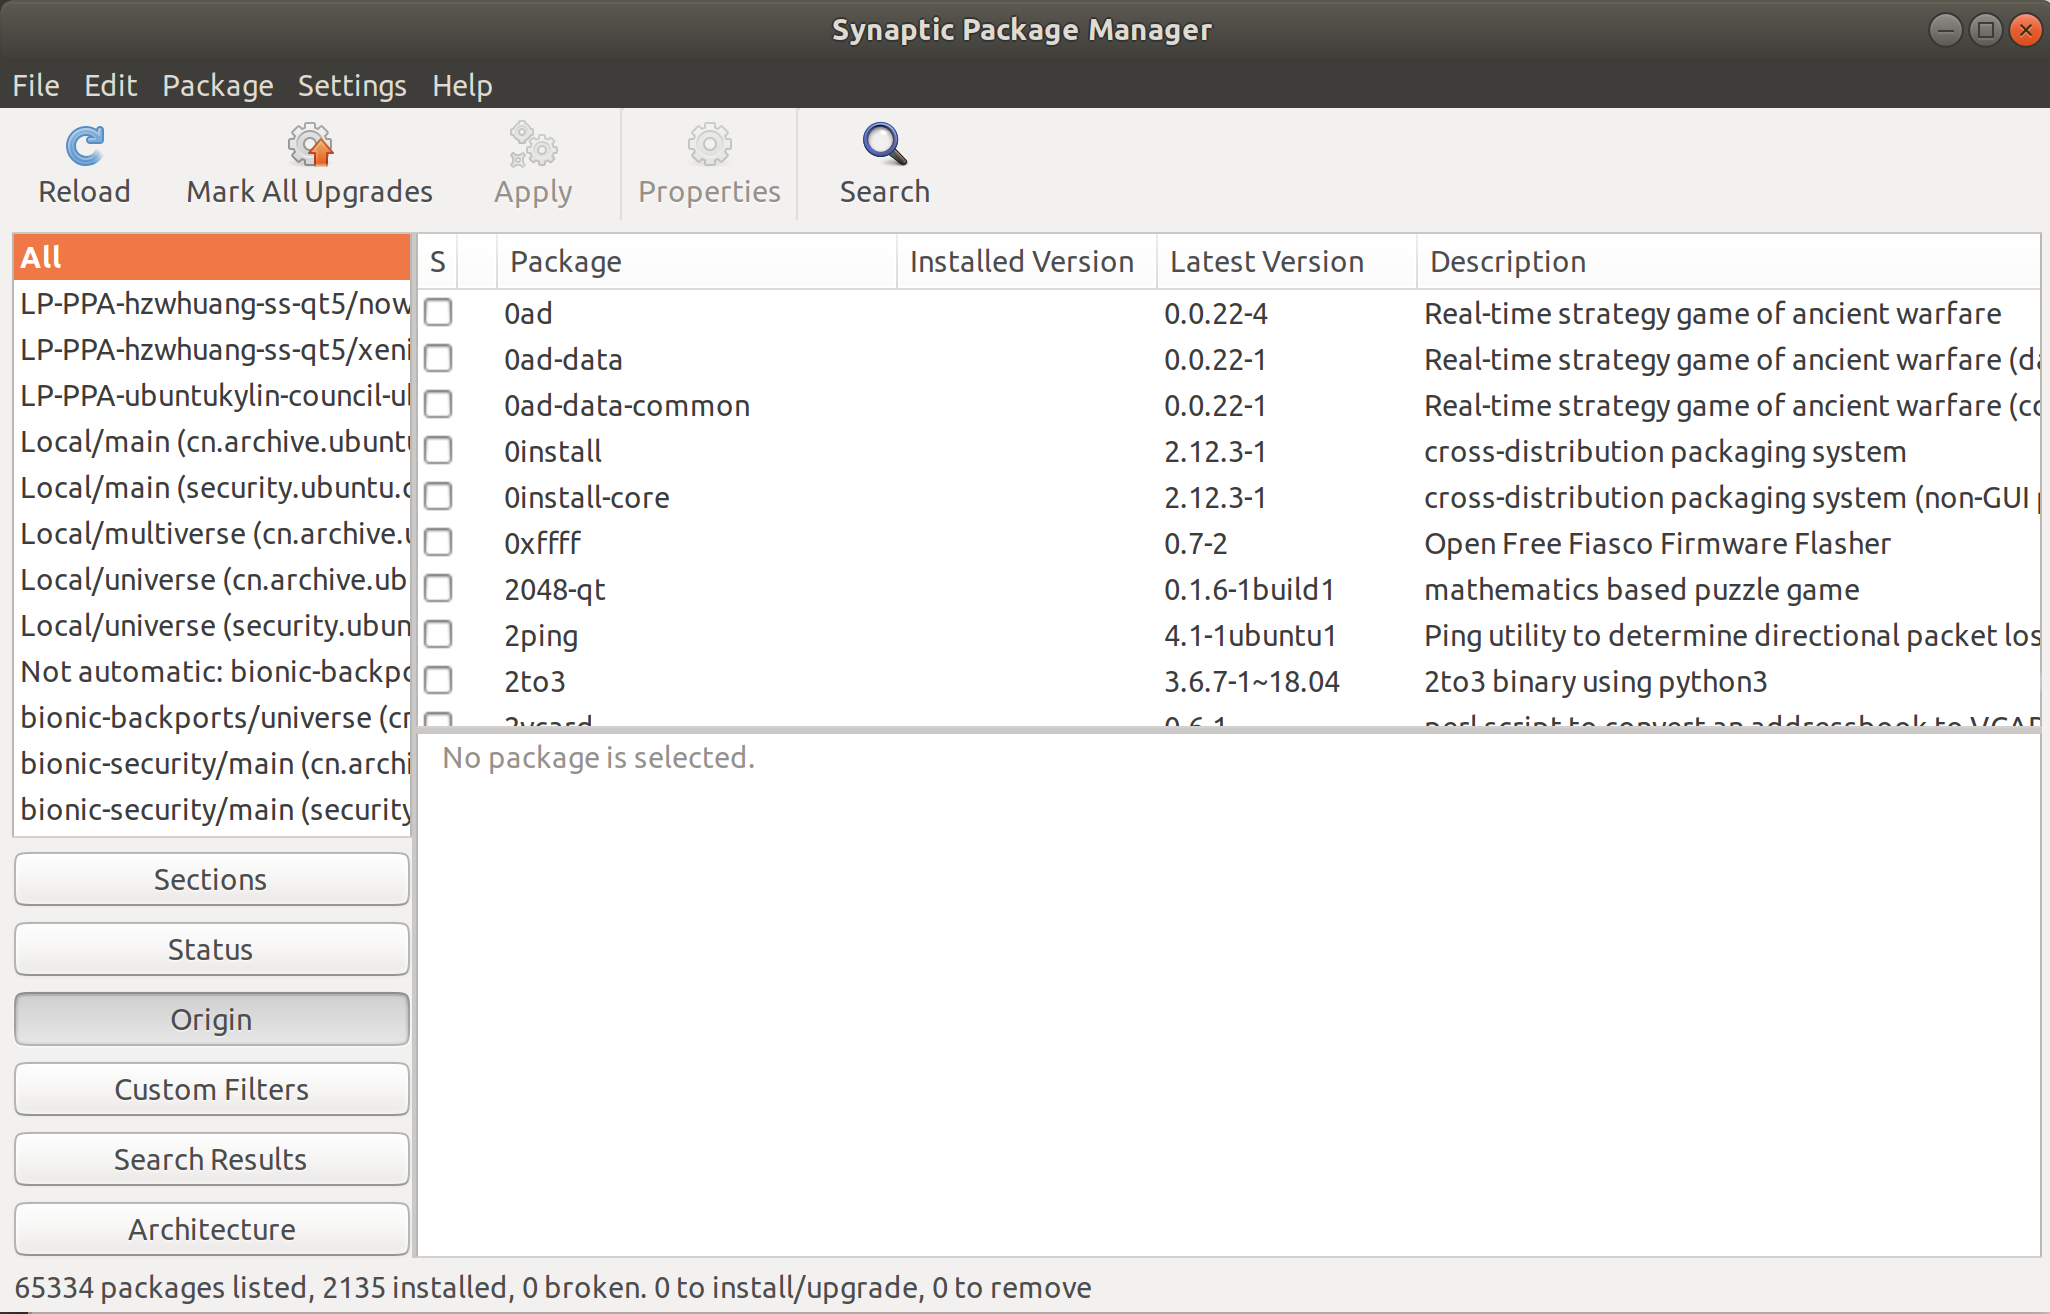
\includegraphics[width=0.45\linewidth]{png/synaptic}
	}
	\hfill
	\subfigure[使用新立得软件包管理器安装软件]{
		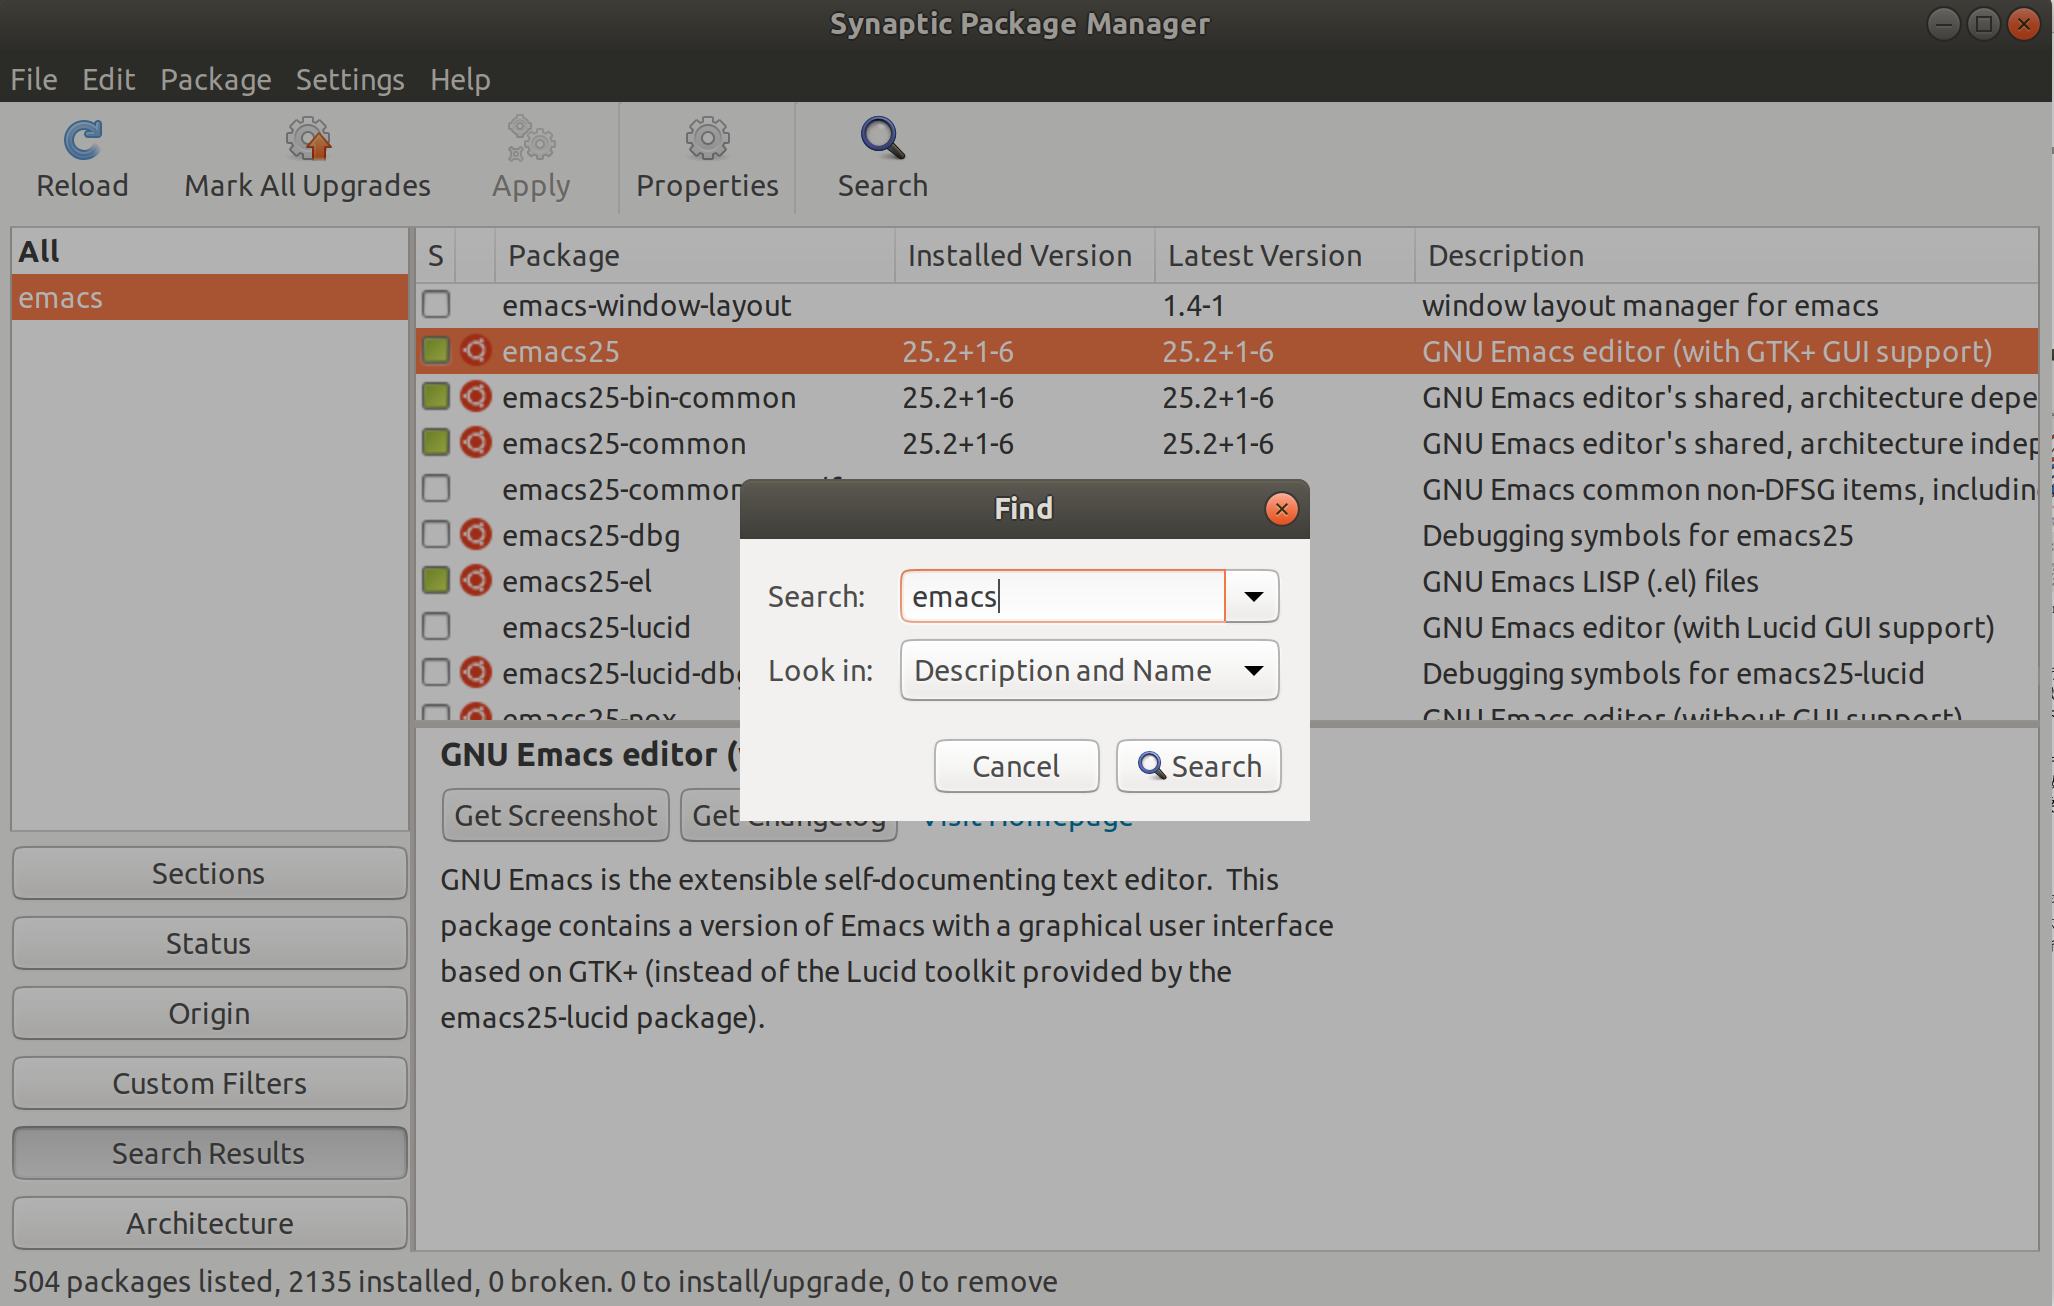
\includegraphics[width=0.45\linewidth]{png/synapticInstall}
	}
	\label{fig:Synaptic}
\end{figure}

\begin{remark}
	不得不提出的是,当你在体验一个新的操作系统的时候,难免会遇到各种各样的问题,
	要学会在使用的过程中进步,牢记常用的命令,养成不会就查的习惯!
\end{remark}






%%% Local Variables:
%%% mode: latex
%%% TeX-master: "../Guide"
%%% End:
